%
% Niniejszy plik stanowi przykład formatowania pracy magisterskiej na
% Wydziale MIM UW.  Szkielet użytych poleceń można wykorzystywać do
% woli, np. formatujac wlasna prace.
%
% Zawartosc merytoryczna stanowi oryginalnosiagniecie
% naukowosciowe Marcina Wolinskiego.  Wszelkie prawa zastrzeżone.
%
% Copyright (c) 2001 by Marcin Woliński <M.Wolinski@gust.org.pl>
% Poprawki spowodowane zmianami przepisów - Marcin Szczuka, 1.10.2004
% Poprawki spowodowane zmianami przepisow i ujednolicenie 
% - Seweryn Karłowicz, 05.05.2006
% Dodanie wielu autorów i tłumaczenia na angielski - Kuba Pochrybniak, 29.11.2016

% dodaj opcję [licencjacka] dla pracy licencjackiej
% dodaj opcję [en] dla wersji angielskiej (mogą być obie: [licencjacka,en])
\documentclass[en]{pracamgr}

\usepackage{amsmath}
\usepackage{amsfonts}
\usepackage{tikz}
\usepackage{hyperref}
\usepackage{cleveref}
\usepackage{float}
\usepackage{booktabs}
\usepackage{xltabular}
\usepackage{ragged2e}
\usepackage{makecell}
\usepackage{multicol}
\usepackage{forest}


\usetikzlibrary{shapes.geometric, arrows.meta, positioning, fit, shadows}
% Dane magistranta:
\autor{Cezary Bednarz}{406099}

% Dane magistrantów:
%\autor{Autor Zerowy}{342007}
%\autori{Autor Pierwszy}{342013}
%\autorii{Drugi Autor-Z-Rzędu}{231023}
%\autoriii{Trzeci z Autorów}{777321}
%\autoriv{Autor nr Cztery}{432145}
%\autorv{Autor nr Pięć}{342011}

\title{Heuristic Portfolio Framework for Quadratic Unconstrained Binary Optimization Problem (QUBO)}
\titlepl{Heurystyczne portfolio algorytmów dla problemu kwadratowej optymalizacji binarnej bez ograniczeń (QUBO)}

%\tytulang{An implementation of a difference blabalizer based on the theory of $\sigma$ -- $\rho$ phetors}

%kierunek: 
% - matematyka, informacyka, ...
% - Mathematics, Computer Science, ...
\kierunek{Computer Science}

% informatyka - nie okreslamy zakresu (opcja zakomentowana)
% matematyka - zakres moze pozostac nieokreslony,
% a jesli ma byc okreslony dla pracy mgr,
% to przyjmuje jedna z wartosci:
% {metod matematycznych w finansach}
% {metod matematycznych w ubezpieczeniach}
% {matematyki stosowanej}
% {nauczania matematyki}
% Dla pracy licencjackiej mamy natomiast
% mozliwosc wpisania takiej wartosci zakresu:
% {Jednoczesnych Studiow Ekonomiczno--Matematycznych}

% \zakres{Tu wpisac, jesli trzeba, jedna z opcji podanych wyzej}

% Praca wykonana pod kierunkiem:
% (podać tytuł/stopień imię i nazwisko opiekuna
% Instytut
% ew. Wydział ew. Uczelnia (jeżeli nie MIM UW))
\opiekun{Marcin Szczuka, Ph.D.\\
  Faculty of Mathematics, Informatics and Mechanics\\
  University of Warsaw
  }
\opiekuni{Łukasz Pawela, Associate Professor\\
  Institute of Theoretical and Applied Informatics\\
  Polish Academy of Sciences\\
  Quantumz.io \\
  }

% miesiąc i~rok:
\date{December 2025}

%Podać dziedzinę wg klasyfikacji Socrates-Erasmus:
\dziedzina{ 
%11.0 Matematyka, Informatyka:\\ 
%11.1 Matematyka\\ 
%11.2 Statystyka\\ 
11.3 Informatyka\\ 
%11.4 Sztuczna inteligencja\\ 
%11.5 Nauki aktuarialne\\
%11.9 Inne nauki matematyczne i informatyczne
}

%Klasyfikacja tematyczna wedlug AMS (matematyka) lub ACM (informatyka)
% taken from https://cran.r-project.org/web/classifications/ACM-2012.html
\klasyfikacja{
Computing methodologies -- Heuristic function construction \\
Computing methodologies -- Ensemble methods \\
Theory of computation -- Discrete optimization \\
Theory of computation -- Optimization with randomized search heuristics
}
% Słowa kluczowe:
\keywords{QUBO, Combinatorial Optimization, Heuristic Portfolio, Metaheuristics, Machine Learning}

% Tu jest dobre miejsce na Twoje własne makra i~środowiska:
% \newtheorem{defi}{Definicja}[section]
% Custom command: typewriter key, equals sign, value. 
% \hangindent ensures multiline values look neat.
\newcommand{\param}[2]{\hangindent=1em \hangafter=1 \texttt{#1} = #2}

% koniec definicji

\begin{document}
\maketitle
%tu idzie streszczenie na strone poczatkowa
\begin{abstract}
This thesis presents an experimental framework for solving the Quadratic Unconstrained Binary Optimization (QUBO) problem, as well as its equivalent formulation, the Ising model. Many hard combinatorial optimization problems, such as airline scheduling or portfolio optimization, can be reduced to the QUBO form. While quantum annealing, a promising approach in quantum computing, may eventually offer advantages for solving such problems, current state-of-the-art classical heuristics continue to achieve superior results. This motivates the exploration of heuristic portfolios, which combine the strengths of multiple metaheuristics to improve performance across different problem instances.
The Heuristic Portfolio Framework classifies parameters of QUBO instances and chooses a set of heuristics that are predicted to perform best. This classifier was trained and validated on a diverse set of problems from well-known benchmark libraries, specifically QUBOLib and MQLib. A Random Forest classifier was employed for its interpretability regarding feature importance. Alongside this, a comparative analysis with the XGBoost classifier was conducted to evaluate classification accuracy and effectiveness. The set of integrated heuristics includes Parallel Tempering, Simulated Bifurcation, and top-performing algorithms from the MQLib library.
Each heuristic was tuned using Bayesian hyperparameter optimization and executed in parallel to maximize resource efficiency. The framework is modular and extensible, supporting the integration of various heuristics, classifiers, and tuning strategies. Experimental results on benchmark instances demonstrate the effectiveness of the portfolio approach. Specifically, the novel, CPU-only \textit{Portfolio of Portfolios} using XGBoost selectors achieved the best results among the tested configurations, securing the best solution in 84\% of the test instances.
\end{abstract}

\tableofcontents
%\listoffigures
%\listoftables

\chapter*{Introduction}
\addcontentsline{toc}{chapter}{Introduction}

In recent years, Quadratic Unconstrained Binary Optimization (QUBO) has emerged as a 
fundamental problem in various fields. The fact that NP-hard problems can be polynomially 
reduced to it, coupled with the simplicity of formulating binary optimization tasks, 
has made it a widely studied and popular problem to solve. Moreover, with the advent of 
quantum computing, QUBO has gained even more attention, as it is well-suited for quantum 
annealers, which exploit quantum phenomena to potentially find solutions more efficiently 
than classical approaches. However, even state-of-the-art quantum annealers still fall short for well
optimized classical approaches, particularly for certain problem instances \cite{tasseff}.

The significance of QUBO problems extends well beyond their theoretical foundations, 
finding practical applications across various domains, including machine learning, 
finance, and logistics. In machine learning, for instance, QUBO is employed to 
enhance model efficiency through feature selection, where it helps in identifying 
the most relevant features while minimizing complexity, as demonstrated in \cite{mucke}. 
In the financial sector, QUBO is applied to portfolio optimization, where the objective 
is to maximize returns while minimizing risk under specific constraints, 
a method effectively utilized in \cite{sakuler}. Similarly, in logistics, QUBO is used 
to optimize vehicle routing, addressing traffic congestion by incorporating constraints 
related to road flow and vehicle density, as explored in \cite{tambunan}.

As noted before, heuristic approaches are still essential for solving QUBO problems, 
and there are numerous metaheuristics that have been proposed to tackle this, 
some working better than others depending on the instance. As studied in \cite{dunning},
and proven in \textit{No Free Lunch Theorems for Optimization} \cite{wolpert1997}, there is no 
single best algorithm for all instances. This motivates the use of algorithm portfolios,
which by combining multiple algorithms, can achieve better performance. In the paper 
\textit{What Works Best When? A Systematic Evaluation of Heuristics for Max-Cut and QUBO} 
\cite{dunning} the authors explore the concept of algorithm portfolios for QUBO problems, 
gathering a set of state-of-the-art metaheuristics from multiple papers and train a 
Random Forest classifier to select the algorithms that probably would get the best results
for a given class of problem instance. 

In this thesis, I would like to explore this idea,
inspired by the work in \cite{dunning}, by implementing the Algorithm Portfolio Framework. 
The main focus will be put on the exploration of combinations of different portfolio components,
which will consist of:
\begin{itemize}
    \item Instances: QUBOLib \cite{qubojl:2023} and MQLib \cite{dunning}
    \item Instance classifier: selected 57 features
    \item Metaheuristic selector: Random Forest \cite{breiman2001} and XGBoost \cite{chen2016xgboost}
    \item Metaheuristic classes: 
    \begin{itemize}
        \item MQLib heuristics \cite{dunning}: Top 8 performers from the library
        \item Metaheuristics.jl \cite{metaheuristics2022}: Particle Swarm Optimization (PSO) \cite{PSO}, Biased Random Key Genetic Algorithm (BRKGA) \cite{BRKGA_review}
        \item Simulated Bifurcation (SB) \cite{SB_original_2019, SB_python}
        \item Parallel Tempering (PT-ICM) \cite{PT_ICM_zhu_2015, PT_rust}
    \end{itemize}  
    \item Metaheuristic parallel execution engine with caching
\end{itemize}

The main advantage of this framework is its easy extensibility. I have explored the interaction
between all components and present a comprehensive evaluation of various configurations. The subsequent chapters
will detail the design of each component, the experimental methodology used for testing, and a thorough analysis
of the obtained results. Ultimately, this thesis aims to demonstrate the efficacy of the portfolio approach and
provide insights into the conditions under which different combinations of classifiers, heuristics, and tuning
strategies yield the best performance for solving QUBO problems.
The resulting module \texttt{QUBOPortfolio.jl} is open-source and available at \url{https://github.com/cezarybednarz/QUBOPortfolio.jl}.

\newpage

\chapter{Background and Related Work}

The challenge of choosing the most suitable algorithm for a given problem instance is not new; it has been recognized since the early days of computing. As early as the 1970s, researchers observed that no single algorithm performs best across all possible inputs and problem classes. This observation laid the foundation for what is now known as the \textit{algorithm selection problem}.

The first formal treatment of this concept was provided by Rice in his seminal work \cite{rice1976}, where he introduced a general framework for algorithm selection. Rice modeled algorithm selection as a mapping between four components: the problem space, the feature space, the algorithm space, and the performance space. The idea was that given a set of problem instances (each described by certain measurable features) and a set of candidate algorithms, one can learn a function that predicts which algorithm will perform best for a particular instance. This framework is still influential today and underpins many modern approaches to automated algorithm selection and portfolio design.

In the decades that followed, the interest in algorithm selection grew alongside advances in both computing power and the complexity of problems tackled by computers. Kotthoff’s comprehensive survey \cite{kotthoff2016} provides an overview of developments in this field, with a particular emphasis on combinatorial search problems. The survey highlights the evolution from manually designed selection rules towards data-driven and machine learning-based approaches, which dominate current research. A recurring theme is the use of instance-specific features, quantitative characteristics that describe the structure or difficulty of a problem instance, to guide algorithm choice.

The need for algorithm selection has historically been motivated by two key observations. First, many hard computational problems, such as NP-hard combinatorial optimization tasks, show significant performance variability across instances. Second, according to the \textit{No Free Lunch Theorems for Optimization} \cite{wolpert1997}, no single algorithm can outperform all others across the entire instance space. These insights make it clear that algorithm portfolios, collections of diverse algorithms coupled with a selection mechanism, offer a principled way to improve robustness and efficiency.

Algorithm selection and portfolios have found applications in numerous domains, including SAT solving, constraint programming, and integer programming. Frameworks such as \textsc{SATzilla} \cite{xu2008} demonstrated the power of machine learning in predicting algorithm performance based on instance features. More recent works extend these ideas to large-scale combinatorial optimization problems, including Quadratic Unconstrained Binary Optimization (QUBO) \cite{dunning}, which is the primary focus of this thesis.

Many real-world challenges in areas like logistics, finance, and engineering can be framed as \textbf{optimization problems}. The goal is simply to find the best possible outcome from a very large set of options. An important category of these is \textbf{discrete optimization}, where the decisions must be whole numbers.

A key field within this area is \textbf{binary optimization}, a central topic in computer science and operations research. The name ``binary'' comes from its main feature: every decision is restricted to just two options, typically written as 0 or 1. This structure is ideal for modeling simple ``yes/no'' choices, such as whether to include an item in a backpack, turn on a specific component, or make an investment.

Formally, a binary optimization problem is about finding a sequence of 0s and 1s (a binary vector $x \in \{0, 1\}^n$) that maximizes or minimizes an objective function $f(x)$ while following a given set of rules, known as constraints. Although each individual choice is simple, the total number of possible solutions grows exponentially with the number of variables ($2^n$). This rapid growth makes finding the perfect solution computationally very difficult. As a result, many famous problems in this class, such as the Traveling Salesman Problem and the Knapsack Problem, are classified as \textbf{NP-hard}.

I will focus on \textbf{QUBO} and other simply reducible problems, like \textbf{Max-Cut} and \textbf{Ising} problems.

In this chapter, I will begin by introducing the theoretical foundations of QUBO and related models, followed by a review of heuristic techniques for solving such problems.
\section{QUBO}
\subsection{Problem Definition}

Quadratic Unconstrained Binary Optimization (QUBO) is the problem of finding a binary vector $x = (x_1, x_2, \ldots, x_n)$, where $x_i \in \{0, 1\}$, that minimizes (or maximizes) a quadratic objective function. A key property of binary variables is that $x_i^2 = x_i$. This allows any linear term $d_i x_i$ to be written as a quadratic term $d_i x_i^2$, which can then be placed on the diagonal of a matrix representation.

This insight allows the QUBO objective function to be expressed compactly in matrix form. In theoretical and formal contexts, the problem is typically defined using a symmetric matrix $Q \in \mathbb{R}^{n \times n}$:

\begin{equation}
  \label{eq:qubo_matrix}
  \min_{x \in \{0, 1\}^n} x^T Q x
\end{equation}

Here, the diagonal elements $q_{ii}$ represent the linear weights of the variables $x_i$, while the off-diagonal elements $q_{ij}$ represent the quadratic interaction strengths between pairs $x_i$ and $x_j$. Since multiplication of variables is commutative ($x_i x_j = x_j x_i$), the contributions from $q_{ij}$ and $q_{ji}$ are combined, which is why a symmetric matrix ($q_{ij} = q_{ji}$) is the natural representation.

It is worth noting that the ability to absorb linear terms onto the diagonal is a unique feature of binary models like QUBO. In the related Ising model, where variables are spins $s_i \in \{-1, 1\}$, the identity is $s_i^2 = 1$, not $s_i^2 = s_i$. Consequently, linear terms in the Ising formulation cannot be merged onto the diagonal and must be treated separately.
For simplicity, this thesis will focus on the \textbf{minimization} problem:
\begin{quote}
    \textbf{QUBO Minimization Problem} \\
    \textit{
Given a symmetric square matrix $Q$ of real-valued coefficients, find the binary vector $x$ that minimizes the quadratic function $f(x) = x^T Q x$.}
\end{quote}
While the symmetric form is standard for theoretical work, for implementation purposes it can be more convenient and memory-efficient to use an upper-triangular matrix. In this convention, the objective function is written as:
\begin{equation}
  \label{eq:qubo_upper_triangle}
  f(x) = \sum_{i=1}^{n} q_{ii} x_i + \sum_{i=1}^{n} \sum_{j=i+1}^{n} q_{ij} x_i x_j
\end{equation}
Any symmetric QUBO formulation can be converted to an equivalent upper-triangular form, and many QUBO solvers are designed to accept this format. In the further chapters I will assume that the QUBO instances are given as an \textbf{upper triangular matrix format}.

The QUBO problem belongs to the class of computationally hard problems.
Specifically, the optimization task of finding the minimum value of the
objective function is classified as \textbf{NP-hard}. The corresponding
decision problem, which asks whether a solution $x$ exists such that $x^T Q x \le k$ for some constant $k$, is formally \textbf{NP-complete}.

The NP-hardness of QUBO is shown through a polynomial-time reduction from
the \textbf{Max-Cut} problem, which is itself a known NP-hard problem. As
the next section will demonstrate, any instance of Max-Cut can be
efficiently converted into an equivalent QUBO instance. This relationship
proves that QUBO is at least as difficult to solve as Max-Cut, confirming its NP-hard status.

Also, it is important to note that in literature the QUBO problem is often referred to as
the Unconstrained Binary Quadratic Programming (UBQP) problem \cite{Quadratic_Programming_tutorial}.

\subsection{Max-Cut}

Max-Cut, also known as Maximum Cut, is a problem defined as one of the original Karp's 21 NP-complete problems \cite{karp}.
The original problem is stated as a decision problem:

\begin{quote}
    \textbf{Max-Cut Decision Problem} \\
    \textit{Given a graph $G$ and an integer $k$, determine whether there is a cut of size at least $k$ in $G$.}
\end{quote}

While the formal definition relates to a decision problem, in practice, I am interested in the corresponding \textbf{optimization problem}: finding a partition of the vertices that maximizes the number of edges in the cut.

\begin{quote}
    \textbf{Max-Cut Optimization Problem} \\
    \textit{Given a graph $G = (V, E)$, find a partition of the vertex set $V$ into two disjoint subsets, $S_1$ and $S_2$, such that the number of edges connecting a vertex in $S_1$ to a vertex in $S_2$ is maximized.}
\end{quote}

Many optimization frameworks, including those for QUBO, are formulated as minimization problems. Therefore, I can equivalently address the Max-Cut problem by minimizing the negative of the cut size. This allows me to use the same solution techniques.

As it turns out, the Max-Cut optimization problem is directly equivalent to a QUBO formulation. This transformation is achieved by assigning a binary variable, $x_i \in \{0, 1\}$, to each vertex $i \in V$, where the value of $x_i$ determines which of the two partitions the vertex belongs to. An edge $(i,j)$ contributes to the cut if and only if its endpoints are in different partitions (i.e., $x_i \neq x_j$). The total size of the cut can therefore be expressed as the sum $\sum_{(i,j) \in E} (x_i - x_j)^2$. Maximizing this sum is equivalent to minimizing its negative, which expands to a quadratic polynomial of the binary variables: the precise definition of a QUBO problem. Because this reduction from an NP-hard problem to QUBO can be done in polynomial time, the QUBO minimization problem is formally classified as \textbf{NP-hard}.

\subsection{Ising Model}

The Ising model is a fundamental concept originating from statistical mechanics, initially proposed to
explain the phenomenon of ferromagnetism \cite{lucas}. It provides a mathematical framework for modeling
the collective behavior of interacting entities, such as atoms in a crystal lattice, where
each entity can exist in one of two states. The goal is to find the configuration of states
that minimizes the total energy of the system.

In the context of optimization, the Ising model is defined as finding the ground state
(minimum energy configuration) of a system of spins.

\begin{quote}
    \textbf{Ising Model Optimization Problem} \\
    \textit{Given a set of interaction couplings $J_{ij}$ and external magnetic fields $h_i$, find the
    configuration of spins $s = (s_1, s_2, \ldots, s_n)$ with $s_i \in \{-1, 1\}$ that minimizes the
    energy function (Ising Hamiltonian) $H(s)$. \\
    The interaction matrix $J$ is symmetric ($J_{ij} = J_{ji}$) and has a zero diagonal ($J_{ii} = 0$).}
\end{quote}
The energy of a given spin configuration is described by the Ising Hamiltonian:
\begin{equation}
    H(s) = - \sum_{i,j} J_{ij} s_i s_j - \sum_{i} h_i s_i
\end{equation}
The components of this equation are:
\begin{itemize}
    \item \textbf{Spins ($s_i$)}: Each variable $s_i$ represents a spin that can be in one of two
    states: ``up'' ($+1$) or ``down'' ($-1$).
    \item \textbf{Couplings ($J_{ij}$)}: The coefficient $J_{ij}$ describes the interaction strength
    between spin $i$ and spin $j$. If $J_{ij} > 0$ (ferromagnetic), the system's energy is lower when
    the spins are aligned ($s_i = s_j$), whereas if $J_{ij} < 0$ (antiferromagnetic), the energy is
    lower when they are anti-aligned ($s_i = -s_j$).
    \item \textbf{External Fields ($h_i$)}: The coefficient $h_i$ represents an external magnetic field
    that influences spin $i$, biasing it towards the up state ($+1$) if $h_i > 0$ or the down state
    ($-1$) if $h_i < 0$.
\end{itemize}
The Ising model is polynomially equivalent to the QUBO formulation. The two models can be converted into one another through a simple linear variable substitution. A problem defined with binary variables $x_i \in \{0, 1\}$ (QUBO) can be translated to one with spin variables $s_i \in \{-1, 1\}$ (Ising) using the transformation $s_i = 2x_i - 1$. Conversely, an Ising problem can be converted to QUBO using $x_i = \frac{s_i + 1}{2}$. This equivalence is particularly significant because many physical systems, including quantum annealers, are naturally described by the Ising model. Therefore, they can be used to solve any problem that can be formulated as a QUBO.

\subsection{QUBO and Ising Model Conversion}
\label{sec:qubo-ising-conversion}

The transformation between the QUBO and Ising models allows any problem expressed in one form to be solved using methods designed for the other. Here, I detail the conversion from the upper-triangular QUBO formulation to the Ising model, as this is a common requirement when interfacing with physics-based solvers. In the next section, I will show the conversion between the QUBO and Ising formulations and vice versa. This will be useful for the implementation part of the thesis.

\paragraph{From QUBO to Ising}
We begin with the QUBO objective function in its upper-triangular form:
\begin{equation}
  f(x) = \sum_{i=1}^{n} q_{ii} x_i + \sum_{i=1}^{n} \sum_{j=i+1}^{n} q_{ij} x_i x_j
\end{equation}
To convert this to the Ising model, we substitute the binary variable $x_i \in \{0, 1\}$ with the spin variable $s_i \in \{-1, 1\}$ using the relation $x_i = \frac{s_i + 1}{2}$. After substitution and algebraic rearrangement, we arrive at an expression that matches the form of the Ising Hamiltonian plus a constant offset.
\begin{equation}
    f(x) = H(s) + C
\end{equation}
The Ising parameters $J_{ij}$ and $h_i$ are derived from the QUBO coefficients $q_{ij}$ as follows:
\begin{align}
    J_{ij} &= -\frac{q_{ij}}{4} \quad \text{for } i < j \\
    h_i &= -\frac{q_{ii}}{2} - \frac{1}{4} \left( \sum_{j > i} q_{ij} + \sum_{j < i} q_{ji} \right)
\end{align}
In the formula for $h_i$, the term $\sum_{j < i} q_{ji}$ refers to the corresponding elements from the lower triangle of the conceptually symmetric QUBO matrix (i.e., $q_{ji} = q_{ij}$). The value of the original QUBO function for a binary solution $x$ is retrieved from the final Ising energy $H(s)$ by the relation $f(x) = H(s) + C$. Since $C$ is a constant, minimizing $H(s)$ is equivalent to minimizing $f(x)$.

\paragraph{From Ising to QUBO}
The reverse conversion is also straightforward. Starting from the symmetric Ising Hamiltonian:
\begin{equation}
    H(s) = - \sum_{i<j} J_{ij} s_i s_j - \sum_{i} h_i s_i
\end{equation}
We apply the transformation $s_i = 2x_i - 1$. After substituting and expanding, we collect the coefficients for the quadratic ($x_i x_j$) and linear ($x_i$) terms. The resulting upper-triangular QUBO matrix $Q$ is:
\begin{align}
    q_{ij} &= -4J_{ij} \quad \text{for } i < j \\
    q_{ii} &= -2h_i + 2 \left( \sum_{j>i} J_{ij} + \sum_{j<i} J_{ji} \right)
\end{align}
The relationship between the models is given by $H(s) = x^T Q x + C'$, where C' is a constant offset. Again, minimizing the QUBO function is equivalent to minimizing the original Ising Hamiltonian.

\subsection{Quantum Annealing}

The QUBO problem's structure makes it an ideal candidate for being solved on specialized hardware, most
notably \textbf{quantum annealers}. These devices are a type of adiabatic quantum computer designed
specifically to tackle optimization problems \cite{hauke2020perspectives}. By leveraging quantum
mechanical effects, such as superposition and quantum tunneling, a quantum annealer attempts to navigate
a complex energy landscape and find the minimum energy state of a system, which directly corresponds to
the optimal solution of a QUBO problem.

The most prominent commercially available quantum annealer is the D-Wave series of quantum processing
units (QPUs) \cite{johnson2011quantum}. These machines are engineered to find the ground state of an
Ising Hamiltonian, which, as established, is equivalent to solving a QUBO. This direct hardware mapping
has generated significant interest in using quantum annealers as a potential accelerator for NP-hard
optimization tasks.

However, the advantage of current quantum annealers is not absolute and is impacted by several practical challenges. A primary issue arises from the limited qubit connectivity of the hardware. The physical qubits on a QPU are not all-to-all connected but are arranged in a fixed, sparse topology, such as the Pegasus or Zephyr architectures in D-Wave's processors \cite{dwave_topologies}. Consequently, the logical graph of a problem often cannot be mapped directly onto the physical qubit layout. To address this, a process known as minor-embedding is required \cite{choi2011minor}, which involves representing a single logical variable with a chain of multiple, strongly-coupled physical qubits.

This embedding process itself introduces significant overhead. Finding an optimal minor-embedding is an \mbox{NP-hard} problem, meaning it must be solved using classical heuristics on a conventional computer before the problem can be run on the QPU. This classical pre-processing step can be a computational bottleneck, diminishing the potential quantum speedup. Furthermore, the quality of the embedding has a direct impact on the final solution's quality. Studies have shown that embedding choices that use fewer physical qubits are, on average, more likely to yield higher-quality solutions and better overall performance \cite{cai2014practical}.

Beyond the structural challenge of embedding, the performance of the annealer is highly sensitive to both its control parameters and environmental noise. The interaction of qubits with their thermal environment, a process known as decoherence, can corrupt the delicate quantum state before the computation is complete. Furthermore, the \textit{annealing schedule}, which dictates the rate of the system's evolution, has a profound influence on the probability of success. A rapid anneal minimizes the system's exposure to environmental noise but increases the risk of diabatic transitions, causing the system to jump to a higher-energy state and miss the optimal solution. Conversely, a slow anneal adheres more closely to the requirements of the adiabatic theorem but extends the system's vulnerability to decoherence \cite{johnson2011quantum}.

Finally, these factors mean that any claims of a quantum advantage must be carefully scrutinized against the best-available classical algorithms, which are themselves a rapidly advancing target. Recent studies show that classical physics-inspired methods, such as those based on simulated bifurcation, can match or exceed the scaling performance of quantum annealers, effectively closing the previously reported performance gaps. Moreover, new and highly efficient classical solvers have demonstrated the ability to outperform state-of-the-art quantum annealers on benchmark problems while also scaling to problem sizes currently intractable for any quantum device. These findings suggest that it is unlikely that the current generation of quantum annealers can demonstrate a definitive practical advantage over continuously improving classical hardware and algorithms \cite{Pawlowski2025_scaling_gap}.

\section{Metaheuristics}

Metaheuristics are a class of approximate optimization algorithms that provide a general-purpose framework for
finding high-quality solutions to difficult, often NP-hard, problems like QUBO. Unlike exact algorithms, 
they do not guarantee finding the globally optimal solution. Instead, their strength lies in their ability
to efficiently navigate vast and complex solution spaces to find near-optimal solutions within a reasonable time. Most metaheuristics operate by balancing between two conflicting objectives: 
exploration of the entire search space to identify promising areas, and exploitation of those areas to 
refine the best solutions found so far. This trade-off is crucial for avoiding local optima, making metaheuristics a cornerstone of modern practical optimization.

\subsection{Tabu Search}
Tabu Search (TS) is a metaheuristic search method using local search methods used for mathematical optimization, first introduced by Fred Glover in 1986 \cite{glover1986}. Unlike standard local search approaches (such as Hill Climbing) which stop when reaching a local optimum, Tabu Search continues the exploration by accepting the best neighbor in the current neighborhood $N(x)$, even if that neighbor worsens the objective function value. To prevent the algorithm from looping back to previously visited solutions and to improve exploration of the solution space, TS maintains a memory structure known as the \textit{tabu list}. This list records recent moves or solution attributes and forbids reversing them for a specific number of iterations, known as the \textit{tabu tenure} \cite{glover1989_TS1}.

In the context of QUBO, a standard move typically consists of flipping a single bit $x_i$. If a bit is flipped, it is added to the tabu list and cannot be flipped back until its tenure expires. However, these prohibitions are not absolute, a mechanism called the \textit{aspiration criterion} allows the algorithm to override the tabu status of a move if it results in a solution better than the best global solution found so far \cite{glover1990_TS2}.

\subsection{Genetic Algorithms}
Genetic Algorithms (GAs) are a class of metaheuristics inspired by Charles Darwin's theory of natural selection.
They are population-based methods that iteratively evolve a set of candidate solutions towards an optimal 
solution. In the context of QUBO, a candidate solution is represented as a binary vector, a string of 0s and 1s 
where each bit corresponds to a variable in the problem. This binary vector is known as a chromosome.

The process begins with an initial population of random solutions (chromosomes). In each iteration, or generation,
the fitness of every solution is evaluated using the QUBO objective function. Solutions with better fitness (i.e.,
lower objective function values in a minimization problem) are more likely to be selected as parents for the next
generation.

New solutions, or offspring, are created from these parents using two primary genetic operators:
\begin{itemize}
    \item \textbf{Crossover (Recombination):} Combines genetic material from two parents to create one or more new 
    offspring. For instance, in a one-point crossover, a random point is selected in the binary strings of two 
    parents, and the segments after that point are swapped.
    \item \textbf{Mutation:} Randomly alters one or more bits (genes) within a chromosome. This introduces
    diversity into the population, helping the algorithm escape local optima and explore new regions of the 
    solution space.
\end{itemize}

The new generation of offspring replaces the old population, and the cycle repeats until a termination condition
is met, such as a fixed number of generations or the convergence of the solution quality. By balancing exploration
(through mutation and diverse parent selection) and exploitation (by favoring high-fitness solutions), GAs can 
effectively search the vast solution spaces characteristic of QUBO problems.

\subsection{Simulated Bifurcation}
\label{sec:simulated-bifurcation}
Simulated Bifurcation (SB) is a modern, physics-inspired metaheuristic designed to solve combinatorial optimization problems, with particular effectiveness on Ising and QUBO models \cite{SB_original_2019}. It translates a discrete optimization problem into the dynamics of a classical system of coupled nonlinear oscillators.

The core idea is to represent the QUBO problem's objective function as the potential energy of this oscillator system. The algorithm then simulates the system's evolution over time, following Hamiltonian mechanics. Initially, the system is energized with a large kinetic term, which is then gradually reduced over time in a process analogous to the \textit{cooling} in Simulated Annealing \cite{kirkpatrick1983}.

As the kinetic energy decreases, the system of oscillators undergoes a bifurcation, where its state rapidly converges to one of several stable equilibrium points. The algorithm is designed such that these final stable states correspond to the optimal or near-optimal solutions of the original QUBO problem. The final spin configuration is determined by the sign of the oscillators' positions.

The Hamiltonian of this system, which describes a network of Duffing oscillators with mass $\Delta^{-1}$ and coupling coefficients $\xi_0 J_{i,j}$, is defined as follows. Note that this formulation corresponds to the Ising model (see Section~\ref{sec:qubo-ising-conversion} for the model conversion), where $J$ represents the interaction matrix:

\begin{equation}
    H_{SB}(\mathbf{x}, \mathbf{y}, t) = \sum_{i=1}^{N} \frac{\Delta}{2} y_i^2 + \sum_{i=1}^{N} \left[ \frac{K}{4} x_i^4 + \frac{\Delta - p(t)}{2} x_i^2 \right] - \frac{\xi_0}{2} \sum_{i=1}^{N} \sum_{j=1}^{N} J_{i,j} x_i x_j
    \label{eq:sb_hamiltonian}
\end{equation}

\noindent Based on this Hamiltonian, the equations of motion governing the time evolution of the state variables (position $x_i$ and momentum $y_i$) are derived as:

\begin{align}
    \dot{x}_i &= \frac{\partial H_{SB}}{\partial y_i} = \Delta y_i \label{eq:sb_motion_x} \\
    \dot{y}_i &= -\frac{\partial H_{SB}}{\partial x_i} = -\left[ K x_i^2 - p(t) + \Delta \right] x_i + \xi_0 \sum_{j=1}^{N} J_{i,j} x_j \label{eq:sb_motion_y}
\end{align}

\noindent where $\Delta$ denotes the detuning frequency, $K$ represents the Kerr non-linearity coefficient, and $p(t)$ serves as the time-dependent pump amplitude that drives the bifurcation process.

The Simulated Bifurcation algorithm has been developed into different variants, offering a trade-off between computational speed and accuracy. The two main variants are the ballistic SB (bSB) and the discrete SB (dSB) \cite{SB_high_performance_2021}. The ballistic variant is optimized for speed and is capable of finding good, approximate solutions in a very short amount of time \cite{SB_kanao_2022_thermal}. On the other hand, the discrete variant, where continuous variables in the equations of motion are replaced by discrete ones, is characterized by higher precision. Although often slower than its ballistic counterpart, dSB is more likely to find the optimal solution due to a quasi-quantum tunneling effect \cite{SB_high_performance_2021}.

A key advantage of the SB algorithm is its inherent parallelism \cite{SB_original_2019}. Since the equations of motion for each oscillator can be updated largely independently, the algorithm works well on massively parallel hardware like GPUs and FPGAs, enabling very fast computation times \cite{SB_original_2019,SB_FPGA_2019}. This hardware implementation is referred to as a Simulated Bifurcation Machine (SBM) \cite{SB_scaling_multi_chip_2021}. Research has shown that SBMs implemented on FPGAs can significantly outperform GPU implementations and other state-of-the-art optimization methods in terms of performance and energy efficiency for certain classes of problems \cite{SB_scaling_multi_chip_2021,SB_FPGA_2019}. For instance, a dSB implementation on a 16-GPU machine successfully solved a one-million-variable problem \cite{SB_high_performance_2021}.

\subsection{Parallel Tempering}
Parallel Tempering is an advanced metaheuristic that builds upon the foundations of Simulated Annealing (SA) \cite{kirkpatrick1983}. While standard SA mimics the physical process of annealing—heating a material and slowly cooling it to reduce defects—it often struggles with the rugged energy landscapes typical of QUBO problems \cite{QUBO_tutorial, Quadratic_Programming_tutorial}. In SA, a single simulation explores the solution space by accepting worse solutions with a probability $P(\text{accept}) = e^{-\frac{\Delta E}{T}}$, where $T$ is a temperature parameter that decreases over time. This allows escape from local optima, but if the cooling is too fast or the barriers are too high, the solver can still get trapped.

Parallel Tempering addresses this by running multiple simulations, known as replicas, in parallel. Each replica simulates the system at a different fixed temperature from a predefined ladder. Replicas at high temperatures can easily cross large energy barriers and explore the solution space globally (exploration), while replicas at low temperatures perform a focused search in promising regions (exploitation).

The key mechanism is the periodic attempt to swap configurations between pairs of replicas at adjacent temperatures. A swap is accepted based on a Metropolis-Hastings criterion. This allows promising solutions discovered by high-temperature replicas to tunnel down to low-temperature replicas for refinement. Conversely, a low-temperature replica trapped in a poor local minimum can escape by swapping its state to a higher temperature.

Advanced variants, such as Parallel Tempering with Isoenergetic Cluster Moves (PT-ICM) \cite{PT_ICM_zhu_2015}, further accelerate exploration in Ising and QUBO problems by performing non-local cluster updates. By exchanging information across temperatures, Parallel Tempering significantly improves the probability of finding the global minimum compared to a standard, single-temperature Simulated Annealing run \cite{PT_ICM_zhu_2015, SA_applications_2019}.
Parallel Tempering is an improvement on top of the Simulated Annealing (SA) algorithm and part of a broader set of temperature-based annealing methods \cite{SA_applications_2019}. It is effective for solving the complex energy landscapes found in QUBO \cite{QUBO_tutorial, Quadratic_Programming_tutorial}. Instead of a single simulation run with a decreasing temperature, Parallel Tempering runs multiple simulations, known as replicas, in parallel. Each replica simulates the system at a different, temperature from a predefined temperature ladder. Replicas at high temperatures can easily cross large energy barriers and explore the solution space globally, while replicas at low temperatures perform a more focused search.

The key step is the periodic attempt to swap the current solutions between pairs of replicas at adjacent temperatures. A swap between a replica at a higher temperature and one at a lower temperature is accepted based on a probability derived from the Metropolis-Hastings criterion. This allows promising solutions discovered by high-temperature replicas to be passed down to low-temperature replicas for further steps. Alternatively, a low-temperature replica that is trapped in a poor local minimum can escape by swapping its configuration with a higher-energy state from a warmer replica.

Advanced variants of this method, such as Parallel Tempering with Isoenergetic Cluster Moves (PT-ICM) \cite{PT_ICM_zhu_2015}, have been developed to further accelerate the exploration of these rugged landscapes, particularly for Ising and QUBO problems. By exchanging information, Parallel Tempering significantly improves the chances of finding the global minimum compared to a standard Simulated Annealing search \cite{PT_ICM_zhu_2015, SA_applications_2019}.

\section{Hyperparameter Optimization}
\label{sec:hyperparameter-optimization}

The formal study of Hyperparameter Optimization began with Eiben et al.'s formalization of the Parameter Setting Problem (PSP) \cite{PSP_eiben1999}, which separated parameter tuning (setting values before the run) from parameter control (adapting values during the run). 

Early approaches to Hyperparameter Optimization relied on simple search strategies. Grid Search evaluates all combinations of parameter values from a predefined grid, while Random Search \cite{RS_bergstra2012} samples parameter configurations uniformly at random. Bergstra and Bengio showed that Random Search often outperforms Grid Search due to the low effective dimensionality of many hyperparameter spaces, most parameters have little impact on performance, and Random Search is more likely to explore the critical dimensions. However, both methods suffer from poor sample efficiency, treating each evaluation as independent and ignoring information from previous trials.

The field advanced with the introduction of model-based optimization techniques. Sequential Model-Based Optimization (SMBO) \cite{SMAC_hutter2011} builds a surrogate model of the objective function and uses it to guide the search toward promising regions. Bayesian Optimization \cite{BAYESIAN_SHAHRIAN2016}, a well-known SMBO method, uses Gaussian Processes to model the performance landscape and acquisition functions like Expected Improvement to balance exploration and exploitation. The SMAC (Sequential Model-based Algorithm Configuration) framework \cite{SMAC_hutter2011} extended this approach to handle categorical and conditional parameters, making it particularly suitable for algorithm configuration problems. Tutorial on Bayesian Optimization \cite{BO_frazier2018} provides a comprehensive overview of the theoretical foundations and practical applications of these methods.

Alternative approaches include racing methods, such as irace \cite{irace_lopez2016}, which use statistical tests to progressively eliminate poorly-performing configurations.

For metaheuristics solving QUBO problems, tuning hyperparameters is an important part of the process. Each algorithm contains multiple interacting parameters that collectively determine its search behavior. The high dimensionality of these parameter spaces, combined with the stochastic nature of the algorithms and the diversity of problem instances, makes manual tuning impractical and motivates the use of automated HPO methods.

\section{Algorithm Portfolio}
\label{sec:algorithm-portfolio}
An Algorithm Portfolio is a framework that leverages a collection of different algorithms to solve a class of 
problems more effectively than any single algorithm could on its own. The concept is rooted in the \textit{No Free Lunch Theorems for Optimization} \cite{wolpert1997}, which state that no single optimization algorithm is 
universally superior for all possible problem instances.

Instead of relying on one solver, a portfolio approach uses an algorithm selection strategy. This typically 
involves a two-stage process:
\begin{enumerate}
    \item \textbf{Offline Training:} A machine learning model, called a \textbf{Selector}, is trained on a large dataset of diverse problem instances. For each instance, a set of descriptive features (e.g., matrix size, 
    density for QUBO) is extracted. The performance of every algorithm in the portfolio is
    benchmarked on these instances. The model learns the mapping between instance features and the best-performing
    algorithm(s).
    \item \textbf{Online Application:} When presented with a new, unseen problem instance, its features are extracted and fed into the trained selector. The selector then predicts which algorithm from the portfolio is 
    most likely to yield the best result. That recommended algorithm is then executed.
\end{enumerate}

This approach can be further enhanced by using parallel computing. Instead of selecting just one best algorithm, the selector can identify a subset of promising algorithms. These can then be run simultaneously on multiple 
processor cores for a fixed time budget. The final solution is the best one found by any of the competing 
algorithms. This parallel portfolio strategy not only capitalizes on the strengths of different algorithms but 
also decreases the risk of a poor algorithm choice, improving both the robustness and performance of the overall 
solution process.

% drugi rozdzial: krotkie wprowadzenie co robie w pracy.
% Co robie od strony technicznej w pracy (na poczatku rozdzialu)
% wybieram metheurystyki, bede robil taki machine learning.
% <kolejna sekcja>
% opisuje metaheurystyki
% <kolejna sekcja>
% czesc machinelearningowa, co to sa za metody machinelearningowe, ekstrakcja cech

% <<<< nowy rodzial>>>
% architektura, software, jaki biblioteki
% <<<<nowy rozdzial>>>>>
% wyniki, analiza

\chapter{Framework Design and Methodology}
\section{The Heuristic Portfolio Concept}
\label{sec:portfolio-concept}
The Heuristic Portfolio Framework (HPF) for QUBO is, in principle, an algorithm portfolio built upon a collection of heuristics commonly used for solving QUBO and its equivalent formulations, such as the Max-Cut problem \cite{karp} and the Ising model \cite{lucas,Quadratic_Programming_tutorial}. The primary focus of this thesis is not the implementation of the individual heuristics, but rather the creation of a framework for systematically testing portfolio configurations.

The central hypothesis is that a portfolio, once trained on a diverse dataset of instances, will outperform any of the heuristics when run individually. This aligns with the \textit{No Free Lunch Theorems for Optimization} \cite{wolpert1997}, which states that no single algorithm is optimal for every problem set. Performance is defined as achieving a superior (i.e., lower) objective value. To achieve this, the framework utilizes machine learning models trained on the structural properties of problem instances \cite{dunning}. In the offline phase the heuristics are first tuned on the training instances, producing a set of optimized hyperparameters, and then the portfolio learns to choose a subset of the tuned heuristics that presumably will perform the best. 

As described in Section~\ref{sec:algorithm-portfolio}, the portfolio operates in two phases: offline training and online application. This section details these two phases and their constituent steps, which include feature extraction, heuristic benchmarking, and the training of the selector and hyperparameter optimization models.

\subsection{Offline Training}

\begin{figure}[h!]
 \centering
    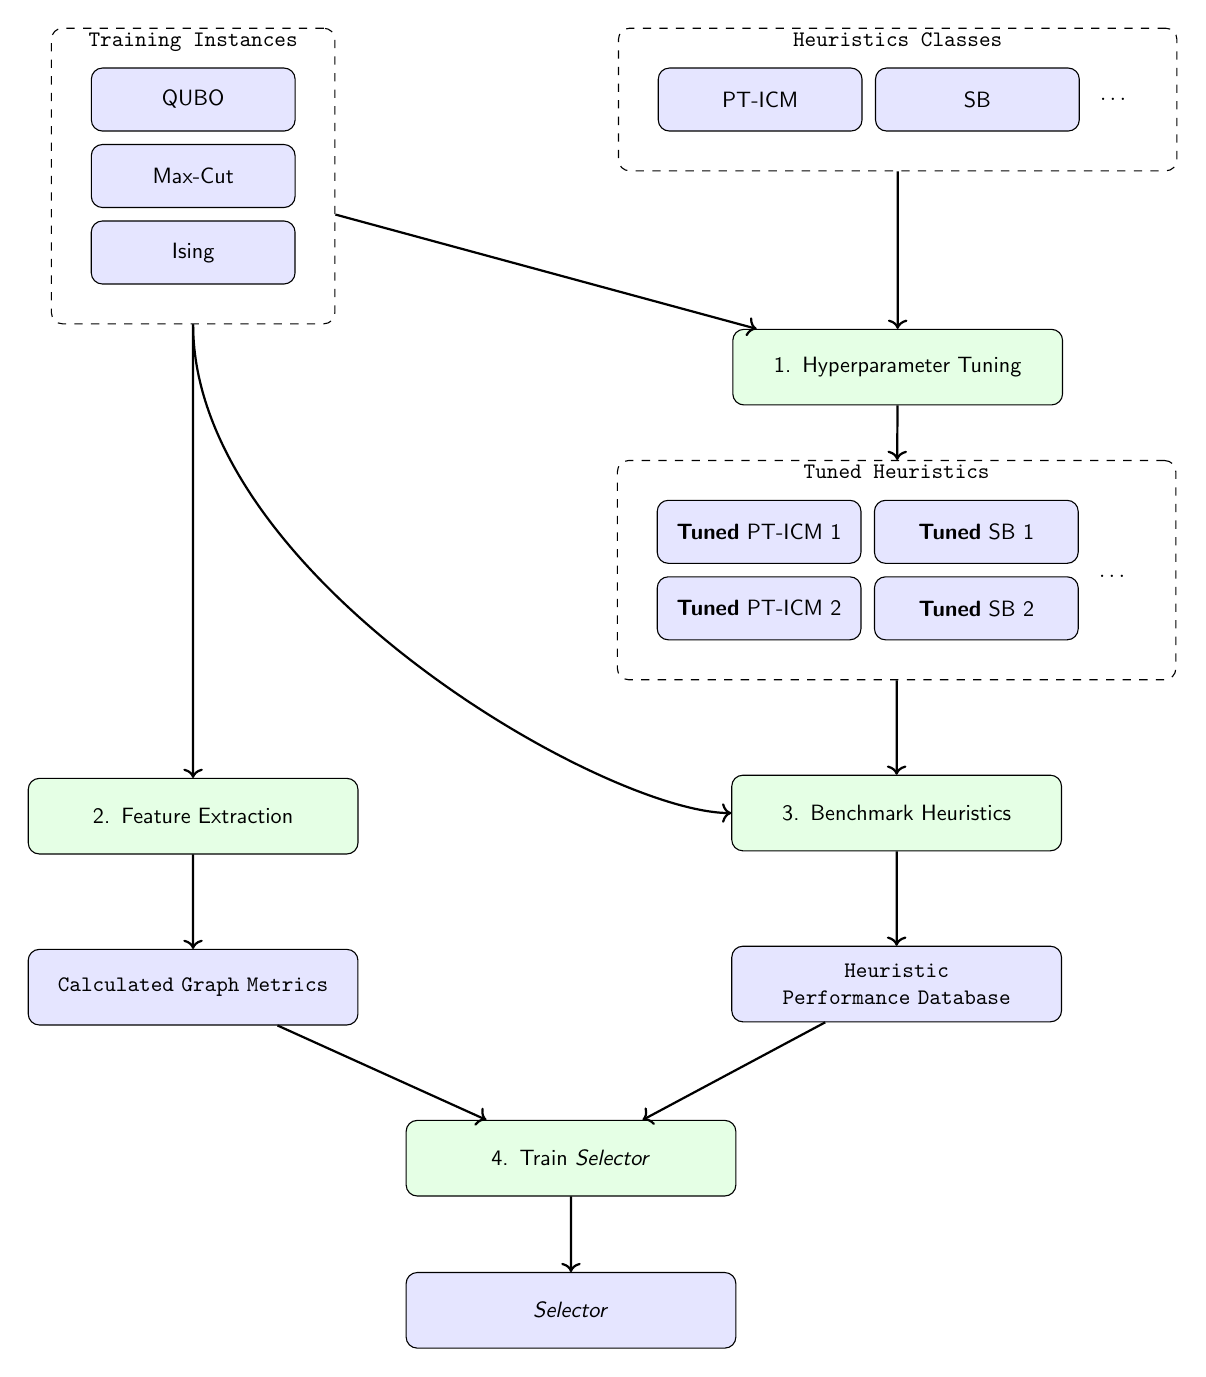
\begin{tikzpicture}[scale=0.8, transform shape,
        data/.style = {
            rectangle,
            draw,
            fill=blue!10,
            rounded corners,
            text width = 4.5cm,
            align = center,
            font = \sffamily,
            minimum height=1.2cm
        },
        process/.style = {
            rectangle,
            draw,
            fill=green!10,
            rounded corners,
            font = \sffamily,
            text width = 5cm,
            align = center,
            minimum height=1.2cm
        },
        fit_node/.style 2 args={
                draw,
                dashed,
                rounded corners,
                inner sep=0.5cm,
                fit=#1,
                label={[anchor=north, inner sep=2pt]north:{\texttt{#2}}}}  ]

        \node (pt_class) [data, text width=3cm, minimum height=1cm] {PT-ICM};
        \node (sb_class) [data, text width=3cm, right=0.2cm of pt_class, minimum height=1cm] {SB};
        \node (etc_class) [right=0.2cm of sb_class] {\dots};

        \node[fit_node={(pt_class)(sb_class)(etc_class)}{Heuristics Classes}] (heuristic_classes) {};

        \node (qubo) [data, text width=3cm, minimum height=1cm, xshift=-9cm] {QUBO};
        \node (maxcut) [data, text width=3cm, below=0.2cm of qubo, minimum height=1cm] {Max-Cut};
        \node (ising) [data, text width=3cm, below=0.2cm of maxcut, minimum height=1cm] {Ising};

        \node[fit_node={(qubo)(maxcut)(ising)}{Training Instances}] (instances) {};
        
        \node (hpt) [process, below=1.5cm of heuristic_classes, yshift=-1cm] {1. Hyperparameter Tuning};

        \node (pt) [data, text width=3cm, below=1.5cm of hpt, xshift=0.5cm, minimum height=1cm, xshift=-2.7cm] {\textbf{Tuned} PT-ICM 1};
        \node (pt2) [data, text width=3cm, below=0.2cm of pt, minimum height=1cm] {\textbf{Tuned} PT-ICM 2};
        \node (sb1) [data, text width=3cm, right=0.2cm of pt, minimum height=1cm] {\textbf{Tuned} SB 1};
        \node (sb2) [data, text width=3cm, below=0.2cm of sb1, minimum height=1cm] {\textbf{Tuned} SB 2};
        \node (etc) [right=0.2cm of sb1, yshift=-0.7cm] {\dots};

        \node[fit_node={(pt)(pt2)(sb1)(sb2)(etc)}{Tuned Heuristics}] (heuristics) {};

        \node (extraction) [process, below=7.2cm of instances]
            {2. Feature Extraction};
        \node (benchmarking) [process, below=1.5cm of heuristics]
            {3. Benchmark Heuristics};
        \node (metrics_dataset) [data, below=1.5cm of extraction, text width=5cm]
            {\texttt{Calculated Graph Metrics}};
        \node (performance_dataset) [data, below=1.5cm of benchmarking, text width=5cm]
            {\texttt{Heuristic Performance Database}};
        \node (selector_training) [process, below=1.5cm of metrics_dataset, xshift=6cm]
            {4. Train \textit{Selector}};
        \node (selector_model) [data, below=1.2cm of selector_training, text width=5cm]
            {\textit{Selector}};
        
        \draw[->, thick] (instances) -- (hpt);
        \draw[->, thick] (heuristic_classes) -- (hpt);
        \draw[->, thick] (hpt) -- (heuristics);
        \draw[->, thick] (instances) -- (extraction);
        \draw[->, thick] (instances.south) .. controls +(0,-4) and +(-2,0) .. (benchmarking.west);
        \draw[->, thick] (heuristics) -- (benchmarking);
        \draw[->, thick] (extraction) -- (metrics_dataset);
        \draw[->, thick] (benchmarking) -- (performance_dataset);
        \draw[->, thick] (metrics_dataset) -- (selector_training);
        \draw[->, thick] (performance_dataset) -- (selector_training);
        \draw[->, thick] (selector_training) -- (selector_model);
    \end{tikzpicture}
\caption{The workflow of the offline training phase. Blue boxes represent data artifacts, while green boxes represent process steps.}
\label{fig:offline-training}
\end{figure}

The offline training process is the most computationally-intensive phase where the \textbf{heuristics are tuned} and the \textbf{\textit{selector} is trained}. As illustrated in Figure~\ref{fig:offline-training}, this process, performed only once, involves four distinct stages.

The first stage is \textbf{1. Hyperparameter Tuning}. This begins with collecting the \texttt{Training Instances} from diverse libraries like QUBOLib and MQLib, alongside the \texttt{Heuristics}  
\texttt{Classes} (such as PT-ICM, SB, Simulated Annealing, etc.). Each heuristic class is subjected to a hyperparameter optimization process across a subset of training instances. For each heuristic class, multiple hyperparameter configurations are explored using Bayesian Optimization (as described in Section~\ref{sec:hyperparameter-tuning-bayesian}). The goal is to identify several well-performing parameter sets for each heuristic class, where each set may specialize on different subsets of the training data. The output of this stage is the \texttt{Tuned Heuristics} collection. This makes the portfolio richer, as the selector can later choose from multiple tuned variants of each heuristic class. The tuning process also can be used to choose hyperparameters that make the heuristics run within a fixed time budget, changing the target energy function to penalize for longer runtimes.

The second stage is \textbf{2. Feature Extraction}. Each problem instance from the \texttt{Training Instances}, no matter if in QUBO, Max-Cut or Ising format, is converted into a Max-Cut graph and analyzed to generate a vector of 57 structural features, following the methodology of \cite{dunning}. The output of this stage is the \texttt{Calculated Graph Metrics} dataset, which maps each instance to its unique feature vector.

The third stage, \textbf{3. Benchmark Heuristics}, is the most computationally demanding. It takes the \texttt{Training Instances} and the \texttt{Tuned Heuristics} as input. Each tuned heuristic variant is executed on every single training instance and its resulting performance (the best objective value found) is recorded. Each heuristic is run 3 times to check for consistency, as some of the heuristics can achieve varying results. This process creates the \texttt{Heuristic Performance Database}, a comprehensive log that maps every combination of (instance, tuned heuristic) to a final performance score. The performance score is 1 if the average of the three runs was in top $k$ best performers for that instance, and 0 otherwise.

With the features and performance data now available, the fourth stage is to \textbf{4. Train \textit{Selector}}. The purpose of this set of models is to predict whether the heuristic assigned to the model will perform in the top \textit{k} heuristics for a given instance. A dedicated binary classification model is trained for \textbf{every} heuristic. Each model, such as a Random Forest \cite{breiman2001} or XGBoost \cite{chen2016xgboost}, learns the mapping from the \texttt{Calculated Graph Metrics} (features) to a binary label indicating whether that specific heuristic will perform in the top $k$ for a given instance. The final output is the \texttt{Selector} model, which consists of this ensemble of binary classifiers that will be used in the online phase to short-list the $k$ best-suited tuned heuristics. It is important to note that the \textit{Selector} can choose multiple tuned variants from the same heuristic class (e.g., both PT-ICM 1 and PT-ICM 2) if they are among the top $k$ performers for a given instance.

\subsection{Online Application}
\label{sec:online-application}

From a top-level perspective, the Heuristic Portfolio Framework functions as a single solver: it accepts a problem instance as input and returns a high-quality solution. Internally, however, this ``online'' application phase involves a multi-step process that uses the models trained offline. The workflow, shown in Figure~\ref{fig:online-application}, begins when a new, unseen problem instance is provided to the framework.

\begin{figure}[h!]
\centering
    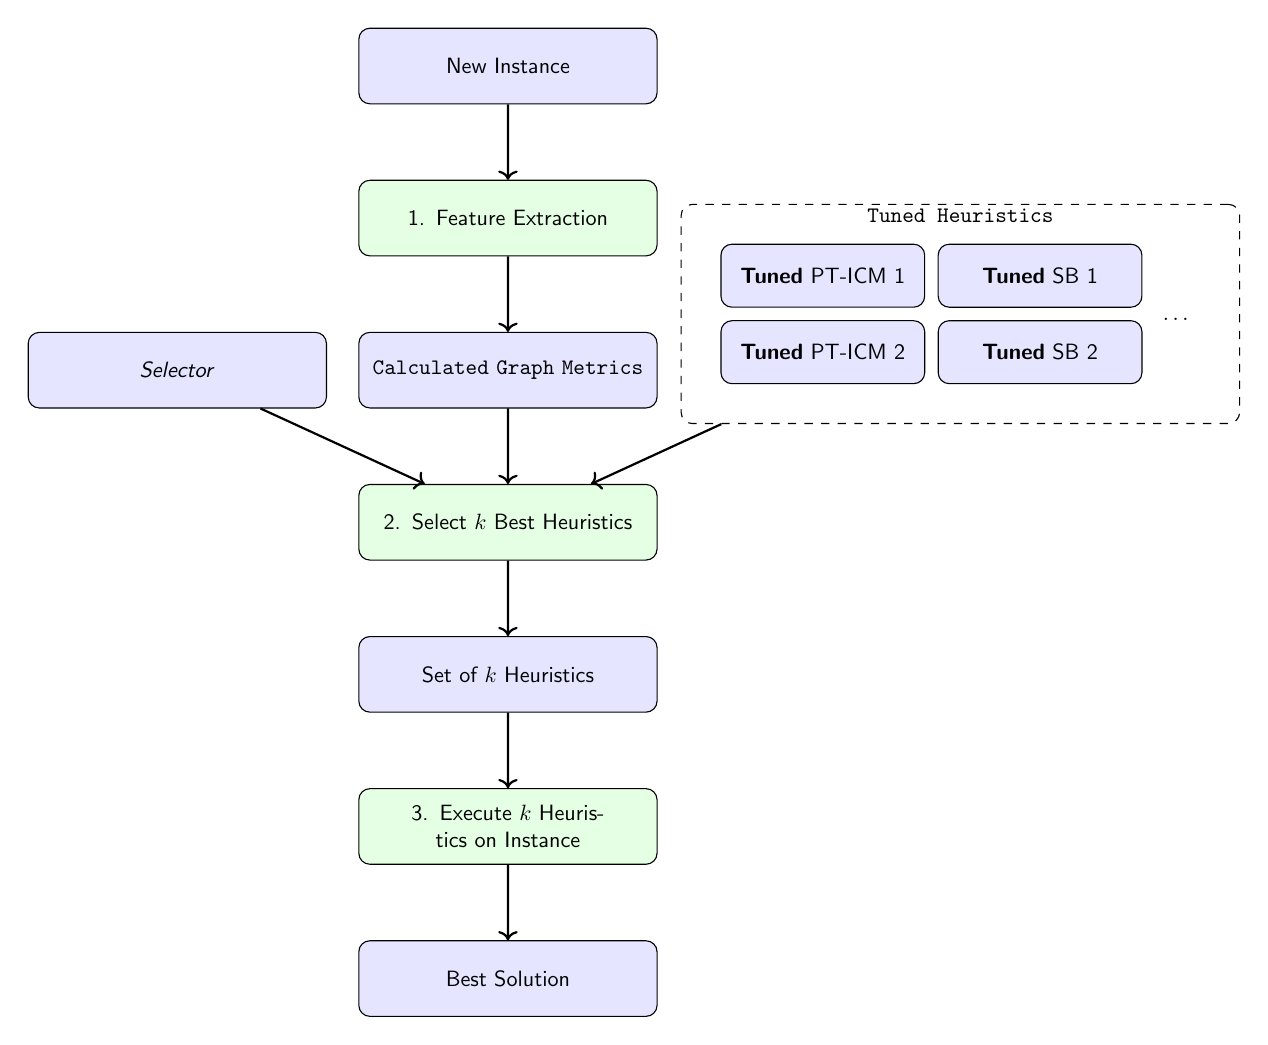
\begin{tikzpicture}[scale=0.8, transform shape,
        data/.style = {
            rectangle,
            draw,
            fill=blue!10,
            rounded corners,
            text width = 4.5cm,
            align = center,
            font = \sffamily,
            minimum height=1.2cm
        },
        process/.style = {
            rectangle,
            draw,
            fill=green!10,
            rounded corners,
            font = \sffamily,
            text width = 4.5cm,
            align = center,
            minimum height=1.2cm
        },
        fit_node/.style 2 args={
                draw,
                dashed,
                rounded corners,
                inner sep=0.5cm,
                fit=#1,
                label={[anchor=north, inner sep=2pt]north:{\texttt{#2}}}}
    ]
    \node (instance) [data]
        {New Instance};
    \node (extraction) [process, below=1.2cm of instance]
        {1. Feature Extraction};
    \node (features) [data, below=1.2cm of extraction]
        {\texttt{Calculated Graph Metrics}};

    \node (pt) [data, text width=3cm, right=1cm of features, yshift=1.5cm, minimum height=1cm] {\textbf{Tuned} PT-ICM 1};
    \node (pt2) [data, text width=3cm, below=0.2cm of pt, minimum height=1cm] {\textbf{Tuned} PT-ICM 2};
    \node (sb1) [data, text width=3cm, right=0.2cm of pt, minimum height=1cm] {\textbf{Tuned} SB 1};
    \node (sb2) [data, text width=3cm, below=0.2cm of sb1, minimum height=1cm] {\textbf{Tuned} SB 2};
    \node (etc) [right=0.2cm of sb1, yshift=-0.7cm] {\dots};
    
    \node[fit_node={(pt)(pt2)(sb1)(sb2)(etc)}{Tuned Heuristics}] (tuned_heuristics) {};

    \node (selector_model) [data, left=0.5cm of features]
        {\textit{Selector}};
    \node (selection) [process, below=1.2cm of features]
        {2. Select $k$ Best Heuristics};
    \node (heuristics) [data, below=1.2cm of selection]
        {Set of $k$ Heuristics};
    \node (execution) [process, below=1.2cm of heuristics]
        {3. Execute $k$ Heuristics on Instance};
    \node (solution) [data, below=1.2cm of execution]
        {Best Solution};

    \draw[->, thick] (instance) -- (extraction);
    \draw[->, thick] (extraction) -- (features);
    \draw[->, thick] (features) -- (selection);
    \draw[->, thick] (tuned_heuristics) -- (selection);
    \draw[->, thick] (selector_model) -- (selection);
    \draw[->, thick] (selection) -- (heuristics);
    \draw[->, thick] (heuristics) -- (execution);
    \draw[->, thick] (execution) -- (solution);
    \end{tikzpicture}
\caption{The workflow of the online application phase. Blue boxes represent data artifacts, while green boxes represent process steps.}
\label{fig:online-application}
\end{figure}

The first step, \textbf{1. Feature Extraction}, involves calculating the same set of 57 structural features for the new instance that were used during the offline training. As shown in Figure~\ref{fig:online-application}, this step produces the \texttt{Calculated Graph Metrics} vector. The computation is designed to be inexpensive, consuming only a small fraction of the total time budget allocated for solving the problem.

Once the features are extracted, the second step, \textbf{2. Select $k$ Best Heuristics}, uses the pre-trained \textit{Selector} model. The selector takes both the \texttt{Calculated Graph Metrics} and the collection of \texttt{Tuned Heuristics} as input. For each tuned heuristic variant, its corresponding binary classifier predicts whether that heuristic is likely to perform in the top $k$ for the given instance. The framework then selects the $k$ heuristics with the highest predicted probabilities, producing a \texttt{Set of $k$ Heuristics} that are expected to perform best.

Finally, in the third step, \textbf{3. Execute $k$ Heuristics on Instance}, these selected heuristics are launched simultaneously, each running on its own processor core with their pre-tuned hyperparameters from the offline training phase. The framework monitors all running processes, and once all heuristics complete their execution, it returns the \texttt{Best Solution}: the lowest objective value found across all $k$ runs. In practice, we use small values of $k$ (between 1 and 4) to balance parallelism and resource usage.

This online architecture allows the framework to function as a black-box solver that adapts its strategy to the unique characteristics of each new problem instance.

\section{Metaheuristics}
\label{sec:metaheuristics}
The main foundation for the framework are the supplied heuristics. As mentioned in the previous chapter, there are many types of heuristic classes with different approaches to optimization. The implemented heuristics include, grouped by package where they were supplied from:
\begin{enumerate}
    \item \textbf{MQLib heuristics}: These are supplied from the MQLib paper \cite{dunning}, where authors implemented 37 most cited QUBO and MAX-CUT solving heuristics in C++ in order to set a standard for heuristic performance benchmarking. The constraints that the authors of \cite{dunning} settled on include hyperparameters set to \textit{values used in empirical testing in their respective papers}, leaving the hyperparameters as an area for future research. This was the main premise for writing this thesis, as I explore the hyperparameter tuning possibilities. Additionally, they all contain runtime-based termination criterion to ensure fair comparison. In practice what that means is that all the heuristics finish in similar time with regard to the instance size. Lastly, all of them are single threaded. As in this thesis there will be other, newer heuristics tested, I decided to include only top 8 best performing heuristics (with highest \textit{mean-of-5} win percentage): \textbf{BUR02, FES02GVP, PAL04T3, FES02GP, FES02GV, PAL04T2, BEA98TS, LU10}. For the specifics of each heuristic, please refer to the original paper \cite{dunning}.

    \item \textbf{Metaheuristics.jl heuristics}: This Julia package \cite{metaheuristics2022} includes a set of metaheuristics for single and multi-objective optimization. Since QUBO is single-objective and unconstrained, I chose \textbf{PSO (Particle Swarm Optimization)} \cite{PSO} and \textbf{BRKGA (Biased Random Key Genetic Algorithm)} \cite{BRKGA_review} from the package.

    \item \textbf{Simulated Bifurcation (SB)}: A physics-inspired metaheuristic for solving Ising and QUBO models \cite{SB_original_2019}. Implemented using the open-source package \cite{SB_python}, which offers four variants:
    \textbf{Ballistic SB (bSB)}, \textbf{Discrete SB (dSB)}, \textbf{Heated ballistic SB (HbSB)}, and \textbf{Heated discrete SB (HdSB)}. For QUBO applications, the \textbf{Discrete} variant was chosen. The package runs on a PyTorch backend on GPU, offering parallelization possibilities using the hyperparameter \texttt{num\_agents}, which denotes the number of threads to analyze in parallel. There also exists another, more efficient solution: Toshiba's Simulated Bifurcation Machine (SBM), which was first designed by Toshiba researchers \cite{SB_goto_2015_bifurcation}, but this solution was omitted due to the high execution costs and closed-source nature.
    \item \textbf{Parallel Tempering (PT)}: The PT-ICM method included in the project is \cite{PT_rust}, a Rust implementation of Parallel Tempering with Isoenergetic Cluster Moves \cite{PT_ICM_zhu_2015}. It is a high-performance implementation that utilizes multi-threading and SIMD instructions for efficient computation. The package allows for tuning several hyperparameters, including the number of replicas, temperature range, and swap frequency.
    \end{enumerate} 

    As for the selection of heuristics, I chose those that are considered either easy to implement in a Julia environment: \textbf{MQLib} and \textbf{Metaheuristics.jl}, as well as those that are considered state-of-the-art solvers: \textbf{SB} for GPU and \textbf{PT-ICM} for CPU \cite{Pawlowski2025_scaling_gap}.

\section{Instance Classifier}
\label{sec:instance-classifier}

The instance classifier is responsible for classifying problem instances through a set of structural features. Following the methodology established in \cite{dunning}, the framework contains a set of exactly the same 57 graph-theoretic metrics to capture the characteristics of each problem instance. The metrics are calculated from an equivalent Max-Cut representation of the QUBO instance. They measure the following properties:
\begin{itemize}
    \item \textbf{Graph Size Metrics}: Logarithm of the number of nodes and edges, providing scale-invariant representations of problem size
    \item \textbf{Degree Statistics}: Average, maximum, and standard deviation of node degrees, characterizing the connectivity distribution
    \item \textbf{Weight Properties}: Statistics of edge weights, including mean, variance, and extremal values
    \item \textbf{Clustering Coefficients}: Measures of local graph density and community structure
    \item \textbf{Spectral Features}: Eigenvalue-based metrics that capture global graph properties
\end{itemize}

This 57-dimensional feature vector is an input to the machine learning models described in Section~\ref{sec:portfolio-concept}. 

The computation of these metrics is performed during both the offline training phase (Section~\ref{sec:portfolio-concept}) and the online application phase (Section~\ref{sec:online-application}). The classification takes a small portion of the total portfolio runtime, and some of the metrics are just approximations.

\section{Hyperparameter Tuning with Bayesian Optimization}
\label{sec:hyperparameter-tuning-bayesian}
In this thesis, I use Bayesian Optimization for hyperparameter tuning. This choice is based on several practical reasons. First, BO is designed for expensive black-box optimization problems where each function evaluation is costly \cite{BO_frazier2018}, the exact scenario we face when benchmarking metaheuristics across hundreds of instances. Second, BO has shown better performance compared to random search and grid search in many algorithm configuration tasks \cite{SMAC_hutter2011}, making efficient use of limited computational budgets through its probabilistic framework. Third, empirical studies have shown that BO-based methods often outperform traditional approaches in tuning metaheuristics, achieving better solution quality with fewer function evaluations. While other methods such as irace \cite{irace_lopez2016} exist in the literature, testing multiple HPO methods would expand the experimental scope beyond the thesis objectives. Given BO's proven track record in similar applications and its theoretical foundation, I adopt it as the hyperparameter optimization method for the framework.

In the framework, all heuristics are treated as black-box functions to be optimized. Each class of heuristics, such as PT-ICM and SB, has a pre-defined set of ranges for every hyperparameter, based on their initial suggested values and exploratory testing. The uniform structure allows us to apply Bayesian Optimization to each heuristic separately within these ranges, tuning their parameters in parallel during offline training. This helps find better configurations for each solver, improving both individual performance and the overall portfolio results.

\section{Selectors} 
\label{sec:selectors}

The problem of selecting the best algorithm for a given instance is a classification task. In this framework, I employ machine learning models, referred to as \textit{Selectors}, to learn the mapping between the structural features of a problem instance and the performance of candidate heuristics. This section outlines the two ensemble learning algorithms used for this purpose: Random Forest and XGBoost. They are still considered state-of-the-art for tabular data classification tasks \cite{grinsztajn2022tree}.

\subsection{Random Forest} Random Forest \cite{breiman2001} is an ensemble learning method that operates by constructing multiple decision trees at training time. It is a bagging (Bootstrap Aggregating) technique, where each tree is trained on a random subset of the data (sampled with replacement).

By aggregating predictions from multiple de-correlated trees trained on random feature subsets, Random Forest reduces variance and overfitting, making it a standard for algorithm selection tasks.

\subsection{XGBoost} XGBoost (Extreme Gradient Boosting) \cite{chen2016xgboost} is a scalable and highly efficient implementation of the gradient boosting framework. Unlike Random Forest, which builds trees in parallel, XGBoost builds an ensemble of trees sequentially. Each new tree is trained to correct the residual errors made by the previous members of the ensemble.

This additive approach allows the model to reduce both bias and variance. XGBoost introduces several advanced features over traditional gradient boosting, including a sparsity-aware algorithm for handling missing data and a regularization term in the objective function (L1 and L2 regularization) to control model complexity. This prevents the model from fitting noise in the training data, a common issue in algorithm selection datasets where the best solver can sometimes be determined by marginal differences in runtime or solution quality.

\subsection{Rationale for Choosing XGBoost} While the seminal MQLib paper \cite{dunning} successfully employed Random Forest for its hyper-heuristic selector, this thesis introduces XGBoost as an alternative and potentially a better candidate for the QUBO portfolio. This is motivated by three factors:

\begin{enumerate} 
    \item \textbf{Probability Calibration:} XGBoost, optimized with \texttt{log\_loss}, often produces better-calibrated probability estimates than Random Forest \cite{niculescu2005predicting}. This is crucial for our framework, which relies on accurate probability rankings to select the top $k$ heuristics.

    \item \textbf{Tabular Data Performance:} Gradient boosting trees are currently considered state-of-the-art for structured tabular data \cite{grinsztajn2022tree}. XGBoost's iterative error correction allows it to capture complex feature interactions more effectively than bagging methods like Random Forest.

    \item \textbf{Tunability:} XGBoost offers a higher degree of tunability compared to Random Forest \cite{probst2018tunability}. This aligns with our offline training strategy, where investing computational resources in hyperparameter optimization yields a more accurate and robust selector for the online phase.
\end{enumerate}

\chapter{Framework Architecture and Software}

The Heuristic Portfolio Framework (HPF) is implemented entirely in the Julia programming language. Julia allows for seamless integration of mathematical optimization, data manipulation, and machine learning, which appears essential for this thesis.

The framework's architecture, as outlined in the \texttt{QUBOPortfolio.jl} module, is organized into several key components:
\begin{itemize}
    \item \textbf{Instance}: Handles loading problem instances from various libraries as well as the conversion between QUBO, Ising and Max-Cut formulations.
    \item \textbf{Metric}: Handles calculating the features of Instances converted to Max-Cut format
    \item \textbf{Heuristics}: Provides a standardized interface for running various solvers, including wrappers for external C++ or Rust binaries and native Julia metaheuristics.
    \item \textbf{Portfolio}: Contains the core logic for the offline training of the machine learning models and the online application of the portfolio.
    \item \textbf{Hyperparameter Optimizer}: Provides methods for heuristic hyperparameter optimization, including random search and model-based approaches (i.e. instance specific tuning).
\end{itemize}
This chapter details the key open-source packages and libraries that underpin each of these components as well as the overall framework design.

\section{Instances representation}

At the base of the framework is the infrastructure for representing the QUBO problem itself. This is primarily handled by the Julia optimization ecosystem, which includes \texttt{JuMP.jl} and \texttt{MathOptInterface.jl}.

\paragraph{JuMP.jl and MathOptInterface.jl} \texttt{JuMP.jl} is a modeling language for mathematical optimization in Julia. While it is much more general than QUBO, it provides the layer upon which many other packages are built. It uses \texttt{MathOptInterface.jl} (MOI) as a solver-agnostic abstraction layer, allowing the framework to interact with different solvers using a single API.

\paragraph{QUBO.jl} The \texttt{QUBO.jl} package \cite{qubojl:2023}, built on top of \texttt{JuMP.jl}, is used as a convenience layer. Its \texttt{QUBOTools.jl} submodule offers standardized in-memory representations of QUBO instances (the $Q$ matrix) and solutions, and it supports multiple file formats for loading and saving QUBO problems that are standard in the industry.

I had to extend the representation with converters between QUBO, MAX-CUT and Ising problems, which are essential for the feature extraction process described in Section~\ref{sec:instance-classifier}, which measures Max-Cut graph properties, and for input to PT-ICM solver \cite{PT_rust}, which takes Ising format.

\section {Instance Libraries}
The instances were supplied from two main libraries:
\begin{itemize}
    \item \textbf{MQLib} \cite{dunning}: A comprehensive library of QUBO and Max-Cut benchmark instances, used in the original Algorithm Portfolio paper \cite{dunning}.
    \item \textbf{QUBOLib} \cite{qubojl:2023}: A more recent library of QUBO instances, provided alongside the \texttt{QUBO.jl} package.
\end{itemize}

The framework supports loading instances from both libraries, loading them into the internal QUBO representation for further processing (alongside Max-Cut and Ising conversions). I needed to implement lazy loading mechanisms to handle the large number of instances efficiently during the offline training phase (the total number and size of instances were much larger than the available RAM during training). This means that instances are only loaded into memory when needed, and released afterward to free up resources.

\section{Metrics}
As mentioned in Section~\ref{sec:instance-classifier}, the framework computes a set of 57 structural features for each problem instance. These features are calculated from the Max-Cut representation of the QUBO instance. The \texttt{SimpleWeightedGraphs.jl} package is used to represent the graph, and most of the metrics are computed using this library.

\section{Heuristics}
The implemented heuristics in the framework consist, as mentioned in Section~\ref{sec:metaheuristics}, of 4 classes: MQLib heuristics, Metaheuristics.jl heuristics, Simulated Bifurcation, and Parallel Tempering. Each of those is wrapped as a standardized interface in the \texttt{Heuristics} module, allowing for uniform execution and parameter passing. This module handles the execution of external binaries (for MQLib and PT-ICM) as well as native Julia implementations (for Metaheuristics.jl). For binary option, it just runs it as a subprocess, passing the instance file and hyperparameters as command-line arguments. The encapsulation also allows for easy caching (see next section) mechanisms to avoid redundant computations during the offline training phase.
The framework runs the set of heuristics in parallel, utilizing every core of the CPU through Julia's standard thread library, utilizing Julia's native \texttt{Threads} library. Additionally, the \texttt{ConcurrentCollections.jl} \cite{concurrentcollectionsjl} package is used for thread-safe data structures when collecting results from parallel executions.

\section{Caching}
Given the computational intensity of the offline training phase, especially during heuristic benchmarking, the framework provides a caching mechanism. This system stores the results of previously executed heuristic runs, indexed by instance, heuristic type and hyperparameter configuration. This prevents redundant computations when the same (instance, heuristic, parameters) combination is encountered multiple times during training. This provided a good way for exploration of different portfolio configurations. The caching had to be implemented thread-safe, as multiple heuristics are run in parallel. Also, the caching stored five results for the same key configuration, as the heuristics are stochastic and can yield different results on different runs. When accessing the cache, the returned value was sampled from the stored results.

The other caching was implemented for the feature extraction process. Since the same instance may be processed multiple times during offline training and online application, the computed feature vectors are cached to avoid recalculating them.

It is important to note that the experimental results presented in Chapter~\ref{chap:experiments} do not utilize this caching mechanism to ensure the integrity of the findings.

\section{Selector}
The selectors are implemented using \texttt{MLJ.jl} \cite{MLJ_2020}, a machine learning framework for Julia that provides interface to machine learning models. Two classifier algorithms were implemented and compared for the selector component:

\paragraph{Random Forest Classifier}
\label{sec:random-forest-classifier}
The Random Forest classifier from the \texttt{DecisionTree.jl} \cite{decisiontreejl} package was selected as the primary selector model, following the methodology in \cite{dunning}. The model uses 500 trees (\texttt{n\_trees=500}) and a minimum leaf size of 1 (\texttt{min\_samples\_leaf=1}). The hyperparameter \texttt{n\_subfeatures} (corresponding to \textit{mtry} in classical Random Forest literature) is tuned using five-fold stratified cross-validation on the training set. This parameter controls the number of features randomly sampled as candidates at each split and is optimized across the range $[1, d]$, where $d$ is the dimensionality of the feature space (57 in our case).

\paragraph{XGBoost Classifier}
As an alternative, the XGBoost classifier from the \texttt{XGBoost.jl} \cite{xgboostjl} package was implemented for comparative analysis. XGBoost is a gradient boosting framework. The implementation uses 100 boosting rounds (\texttt{num\_round=100}) with a learning rate of 0.3 (\texttt{eta=0.3}). The objective function is set to \texttt{multi:softprob}. The \texttt{max\_depth} hyperparameter, which controls the maximum depth of each tree, is tuned via five-fold stratified cross-validation over the range $[3, 10]$.

\subsection{Training Procedure}
Both classifiers use \texttt{MLJ.jl}'s \texttt{TunedModel} wrapper, which automates the hyperparameter optimization process. The tuning uses a grid search strategy with 5 resolution points, using accuracy as the evaluation metric. Stratified cross-validation ensures that each fold maintains the same class distribution as the original dataset, which is important given the multi-label nature of the selection problem. After tuning, the best-performing model configuration is retrained on the entire training set (\texttt{train\_best=true}), producing the final selector model used in the online application phase.

As mentioned in Section~\ref{sec:selectors}, the framework treats each heuristic independently, training a separate selector for each one.

\section{Hyperparameter Optimizer using Hyperopt.jl}
\label{sec:hyperparameter-tuning-hyperopt}
The Hyperparameter Optimizer is built using the \texttt{Hyperopt.jl} package \cite{bagge2018hyperopt}. It uses the BOHB (Bayesian Optimization and Hyperband) algorithm \cite{falkner2018bohb}. BOHB is efficient because it combines two strategies: it uses Hyperband \cite{li2017hyperband} to quickly stop configurations that perform poorly, and it uses Bayesian Optimization to learn which parameters are likely to work best based on previous results.

The current version of BOHB in \texttt{Hyperopt.jl} only supports continuous (decimal) search spaces. To handle other types of parameters, the framework converts the inputs as follows:
\begin{itemize}
    \item \textbf{Continuous Parameters:} These are used directly (e.g., for probabilities or heating coefficients).
    \item \textbf{Integer Parameters:} The optimizer selects a continuous decimal value $\tilde{p}$, which is then rounded to the nearest integer $p = \lfloor \tilde{p} \rceil$ before running the heuristic.
    \item \textbf{Categorical Parameters:} These are handled as indices. For a list of options, the optimizer selects a decimal number. This number is rounded and used as an index to pick an item from the list.
\end{itemize}

The optimization process is controlled by a parameter defining the number of iterations (steps), which determines how many distinct hyperparameter configurations the BOHB algorithm will evaluate. 

The optimization tries to minimize the following loss function:

\begin{equation}
    \mathcal{L}(\theta) = \frac{1}{|\mathcal{S}|} \sum_{i \in \mathcal{S}} E(i, \theta) + \rho \cdot \max\left(0, \max_{i \in \mathcal{S}} \tau(i, \theta) - t_{\text{limit}}\right)
\end{equation}

In this formula:
\begin{itemize}
    \item $\theta$ is the set of hyperparameters.
    \item $\mathcal{S}$ is the subset of training instances.
    \item $E$ is the energy (objective value) found by the heuristic.
    \item $\tau$ is the time the heuristic took to run.
    \item $t_{\text{limit}}$ is the maximum allowed time.
    \item $\rho$ is a penalty added if the time limit is exceeded.
\end{itemize}
This formulation implies that if the heuristic exceeds the time limit, a penalty is added to the loss. A linear penalty is applied rather than a fixed, large constant penalty. As noted by \cite{gelbart2014bayesian}, assigning a large constant value to constraint violations introduces sharp discontinuities in the objective function. Since Gaussian Processes rely on smoothness assumptions, they struggle to model such discontinuities, which can lead to poor optimization performance. This linear penalty encourages the optimizer to identify hyperparameters that achieve good solutions while respecting time limits.

To create a diverse portfolio, the framework runs multiple optimization sessions in parallel. Each session uses a different random subset of training data. This results in several different tuned versions of each heuristic.

\chapter{Experimental Results}
\label{chap:experiments}

The experiments validate whether a machine learning guided portfolio can outperform individual solvers on diverse QUBO instances. Results are presented in two main parts: First, a reproduction study of the MQLib methodology \cite{dunning}, as well as analysis of different portfolio variants and selection strategies. Second, an extended evaluation using hyperparameter tuning mechanisms, demonstrating the added value of automated parameter optimization. 

\section{Experimental Setup}

The experiments were conducted on a single N1 VM rented from Google Cloud with the following specifications:
\begin{itemize}
    \item \textbf{CPU}: 32 vCPUs (Intel Haswell)
    \item \textbf{Memory}: 40 GB RAM
    \item \textbf{GPU}: NVIDIA Tesla T4 (16 GB VRAM)
    \item \textbf{Storage}: 100 GB Balanced Persistent Disk	
    \item \textbf{Operating System}: Debian GNU/Linux 12 (bookworm)
    \item \textbf{Julia Version}: 1.11.6
\end{itemize}
The other specifications are available in Appendix~\ref{ch:reproducibility}.

Since the SB and TAMC packages run as external subprocesses, standard Julia profiling tools could not be used. Also, because I aim to treat these heuristics as black boxes, I could not modify their source code to add measurement tools. Therefore, resource usage was estimated based on the total time the subprocess took to finish. CPU usage was calculated by multiplying this time by the number of threads used (for example, the \texttt{threads} parameter for TAMC). For GPU usage, the method is simple: if a heuristic uses the GPU, the entire run time counts as GPU time. This method gives a safe upper estimate of resource usage, ensuring the reported costs reflect the maximum possible resource allocation.

\section{Dataset Composition}

For the experimental evaluation, a subset of benchmark instances was selected from the MQLib \cite{dunning} and QUBOLib \cite{qubojl:2023} libraries. Only instances with at most 20,000 nodes were considered, as larger instances would exceed the sensible time for benchmarking, as for instances greater than this the single heuristics run for SB ran more than 800 seconds. The instances were chosen as a random subset of the corresponding datasets.

The final dataset consists of 600 instances distributed as follows:
\begin{itemize}
    \item \textbf{Training set (MQLib)}: 400 instances from MQLib
    \item \textbf{Test set (MQLib)}: 100 instances from MQLib
    \item \textbf{Test set (QUBOLib)}: 100 instances from QUBOLib
\end{itemize}

This split ensures that the machine learning models are trained exclusively on MQLib data, while being evaluated on both in-distribution (MQLib test set) and out-of-distribution (QUBOLib) instances. The out-of-distribution evaluation is important for assessing the generalization capability of the trained selector and hyperparameter optimizer. The number of variables and density of the train and test instances could be seen in Figure~\ref{fig:instance-distributions}. 

The 100 QUBOLib \cite{qubojl:2023} test instances were chosen with equal split from the following four categories: \textit{arXiv-1903-10928-3r3x}, \textit{arXiv-1903-10928-5r5x}, \textit{arXiv-2103-08464-3r3x}, and \textit{qplib}.

\begin{figure}[h!]
    \centering
    \begin{minipage}{0.32\textwidth}
        \centering
        \includegraphics[width=\linewidth]{../plots/MQLib_Training_Instances.png}
    \end{minipage}
    \hfill
    \begin{minipage}{0.32\textwidth}
        \centering
        \includegraphics[width=\linewidth]{../plots/MQLib_Test_Instances.png}
    \end{minipage}
    \hfill
    \begin{minipage}{0.32\textwidth}
        \centering
        \includegraphics[width=\linewidth]{../plots/QUBOlib_Test_Instances.png}
    \end{minipage}
    \caption{Instance distributions used for training and evaluation. The density means the number of non-zero elements in the QUBO matrix divided by the total number of elements.}  \label{fig:instance-distributions}
\end{figure}

\section*{Experiment 1: MQLib Reproduction}
\addcontentsline{toc}{section}{Experiment 1: MQLib Random Forest vs XGBoost}

This part of experiments focuses on reproducing the results from the original MQLib paper \cite{dunning}. The reproduction is slightly smaller, meaning that:
\begin{itemize}
    \item Only top 8 heuristics are used (see Section~\ref{sec:metaheuristics})
    \item The heuristics were run 3 times per instances, instead of 5, and the mean performance was recorded (mean-of-3).
    \item The training set consists of 400 instances from MQLib, while the test set contains 100 unseen MQLib instances.
\end{itemize}

I ran the top 8 best performing MQLib heuristics (see Section~\ref{sec:metaheuristics}) on the train instances with selectors set as Random Forest and XGBoost with hyperparameters set as in Paragraph~\ref{sec:random-forest-classifier}. I ran them on both MQLib and QUBOLib test instances. The results on MQLib test instances are presented in Table~\ref{tab:heuristic-performance}. 

The table shows the number of instances where each heuristic achieved the best solution (\textbf{Best}), the number of instances where it was the only heuristic to achieve the best solution (\textbf{Only}), the number of instances where it performed worst (\textbf{Worst}), the average time taken per instance (\textbf{Avg Time (s)}), and the total core hours consumed (\textbf{Core Hours}). In this instance all the heuristics are single threaded so the core hours is just total time.

As expected, both portfolio configurations outperform individual heuristics, with the Random Forest selector achieving 68 best performances out of 100 instances. The XGBoost selector performs comparably, with 67 best performances, but slightly more unique bests (5 vs 3). 

% /experiments/experiment1/vanilla_mqlib_random_forest_xgboost.jl
\begin{table}[h!]
\centering
\caption{Comparison of Heuristic Performance on MQLib Test Instances.\\}
\label{tab:heuristic-performance}
\resizebox{\textwidth}{!}{%
\begin{tabular}{l|rrr|rr}
\toprule
\textbf{Heuristic} & \textbf{Best} & \textbf{Only} & \textbf{Worst} & \textbf{Avg Time  (s)} & \textbf{Core Hours} \\
\midrule
\textbf{Portfolio MQLib RandomForest top\_k=1} & 68 & 3 & 33 & 1.682 & 0.0467 \\
\textbf{Portfolio MQLib XGBoost top\_k=1} & 67 & 5 & 33 & 1.569 & 0.0436 \\
FESTA2002GPR & 61 & 5 & 44 & 1.377 & 0.0382 \\
FESTA2002GVNS & 61 & 4 & 36 & 1.397 & 0.0388 \\
BURER2002 & 58 & 11 & 38 & 1.395 & 0.0387 \\
PALUBECKIS2004bMST3 & 55 & 1 & 33 & 1.671 & 0.0464 \\
FESTA2002VNSPR & 48 & 0 & 33 & 1.390 & 0.0386 \\
LU2010 & 48 & 0 & 39 & 1.483 & 0.0412 \\
BEASLEY1998TS & 46 & 2 & 70 & 1.381 & 0.0384 \\
PALUBECKIS2004bMST2 & 45 & 1 & 39 & 1.387 & 0.0385 \\
\bottomrule
\end{tabular}
}
\end{table}

The results on QUBOLib test instances are presented in Table~\ref{tab:heuristic-performance-qubolib}. Here we can see that both portfolio configurations fall behind the top individual heuristics. This may be due to the distributional shift between MQLib training instances and QUBOLib test instances, which could affect the selector's ability to generalize. This aspect was not explored by the authors of \cite{dunning}, as they only tested on MQLib instances. This shows that the selectors were not able to generalize well to out-of-distribution instances. The XGBoost selector slightly outperforms the Random Forest in this case, achieving 12 best performances compared to 9, while the single best heuristic (LU2010) achieves 97 best performances.

% /experiments/experiment1/vanilla_mqlib_random_forest_xgboost.jl
\begin{table}[h!]
\centering
\caption{Comparison of Heuristic Performance on QUBOLib Test Instances.\\}
\label{tab:heuristic-performance-qubolib}
\resizebox{\textwidth}{!}{%
\begin{tabular}{l|rrr|rr}
\toprule
\textbf{Heuristic} & \textbf{Best} & \textbf{Only} & \textbf{Worst} & \textbf{Avg Time (s)} & \textbf{Core Hours} \\
\midrule
LU2010 & 97 & 43 & 7 & 5.651 & 0.1570 \\
FESTA2002VNSPR & 52 & 2 & 7 & 1.784 & 0.0495 \\
PALUBECKIS2004bMST2 & 37 & 1 & 23 & 1.748 & 0.0486 \\
FESTA2002GPR & 19 & 0 & 18 & 1.849 & 0.0514 \\
PALUBECKIS2004bMST3 & 12 & 0 & 7 & 3.353 & 0.0931 \\
\textbf{Portfolio MQLib XGBoost top\_k=1} & 12 & 0 & 7 & 1.861 & 0.0517 \\
FESTA2002GVNS & 10 & 0 & 7 & 1.913 & 0.0531 \\
\textbf{Portfolio MQLib RandomForest top\_k=1} & 9 & 0 & 7 & 1.850 & 0.0514 \\
BEASLEY1998TS & 9 & 0 & 72 & 1.852 & 0.0515 \\
BURER2002 & 7 & 0 & 9 & 1.821 & 0.0506 \\
\bottomrule
\end{tabular}
}
\end{table}

These results highlight a limitation of the trained selectors: while they are particularly good at selecting algorithms for instances similar to the training set, they struggle to generalize to unseen problem classes with different structural characteristics. For out-of-distribution instances like those in QUBOLib, a robust single heuristic such as LU2010 proves to be a more reliable choice than the portfolios.

\section*{Experiment 2: Hyperparameter Optimization}
\addcontentsline{toc}{section}{Experiment 2: Hyperparameter Optimization}
\label{sec:experiment-2-hpo}

In this experiment, I evaluate the impact of hyperparameter optimization on individual heuristics. Each heuristic from Section~\ref{sec:metaheuristics} was tuned using Bayesian Optimization (see Section~\ref{sec:hyperparameter-tuning-bayesian}) on the training set of 400 MQLib instances. The tuning process aimed to identify hyperparameter configurations that improve the average performance across the training instances. In this section, I focus specifically on the Simulated Bifurcation (SB) and TAMC (PT-ICM) heuristics. It is important to note that from now on, I will not target the Metaheuristics.jl implementations, as they showed inferior performance on the test set: see Table~\ref{tab:heuristic-performance-experiment3}, where the BRKGA and PSO heuristics position themselves at the bottom of the table. The tuned versions of Metaheuristics.jl also showed no significant improvements.

A primary objective of this thesis is to demonstrate how, without modifying the internals of the heuristics (treating them as black boxes), we can adjust them to perform optimally on specific training instances. The Hyperparameter Optimization component of this thesis focuses on two goals: minimizing the resulting energy and adhering to execution time limits.

To demonstrate the performance improvement, it was necessary to establish a fixed time limit. As a reference, I aimed for the tuned heuristics to operate within runtimes similar to those of the default heuristics (see Heuristics Card in Table~\ref{tab:heuristic-model-card}). The distributions of execution times for the default SB and TAMC heuristics on the training dataset are presented below in Figure~\ref{fig:default-execution-times}.

\begin{figure}[h!]
    \centering
    \begin{minipage}{0.48\textwidth}
        \centering
        \includegraphics[width=\linewidth]{../plots/training_execution_time_histogram_sb.png}
    \end{minipage}
    \hfill
    \begin{minipage}{0.48\textwidth}
        \centering
        \includegraphics[width=\linewidth]{../plots/training_execution_time_histogram_tamc.png}
    \end{minipage}
    \caption{Execution time distributions for default SB (left) and TAMC (right) heuristics on the training dataset. The distributions exhibit a tail characteristic of log-normal distributions. The vertical red lines indicate the 95th percentile.} \label{fig:default-execution-times}
\end{figure}

As can be seen in Figure~\ref{fig:default-execution-times}, both distributions are left-skewed, resembling log-normal distributions. Assuming they follow a log-normal distribution, I calculated the 95th percentile of both datasets to serve as the time limit for the hyperparameter optimization. For SB, the 95th percentile corresponds to approximately 82.7 seconds, while for PT-ICM, it is approximately 184.4 seconds (as indicated by the upper bounds in the figures). Consequently, the corresponding time limits were set to 82 seconds for SB and 184 seconds for PT-ICM during the hyperparameter optimization process (see Section~\ref{sec:hyperparameter-tuning-hyperopt} for details on the time limit parameter $t_{\text{limit}}$ in the loss function).

The Bayesian Optimization process ran for 75 iterations, and each new hyperparameter set was trained on a random subset of 25 training instances. This approach ensures that the optimization process fits within reasonable computational budget and hopefully captures diverse instance characteristics, possibly achieving different local minima in the hyperparameter space. The penalty for breaching the time limit $\rho$ is set to 100.0, meaning each second over the time limit adds 100.0 to the loss function. Experimentally this value provided a good balance between solution quality and fitting the time constraints.

\subsection*{TAMC (PT-ICM) Hyperparameter Tuning Results}

\begin{table}[h!]
\centering
\caption{Comparison of TAMC (PT-ICM) Hyperparameters: Default, Search Range, and Tuned Sets.\\}
\label{tab:tamc-hyperparameters}
\resizebox{\textwidth}{!}{%
\begin{tabular}{l|l|l|l|l}
\toprule
\textbf{Parameter} & \textbf{Default Value} & \textbf{Search Range} & \textbf{Tuned Set 1} & \textbf{Tuned Set 2} \\
\midrule
\texttt{num\_sweeps} & 2000 & $[25, 500]$ & 204 & 181 \\
\texttt{warmup\_fraction} & 0.5 & $[0.1, 0.9]$ & 0.407 & 0.674 \\
\texttt{lo\_beta} & 1.0 & $[0.5, 1.5]$ & 0.843 & 1.207 \\
\texttt{num\_replica\_chains} & 2 & $\{2, 4, 8, 16, 32, 64, 128, 256\}$ & 16 & 64 \\
\texttt{beta\_min} & 0.2 & $[0.1, 1.0]$ & 0.309 & 0.145 \\
\texttt{beta\_max} & 5.0 & $[2.0, 10.0]$ & 4.747 & 6.364 \\
\texttt{num\_beta} & 32 & $[16, 64]$ & 52 & 54 \\
\texttt{icm} & true & Fixed & true & true \\
\texttt{threads} & 1 (changed to 4 during testing) & Fixed & 4 & 4 \\
\texttt{sample\_states} & 32 & Fixed & 32 & 32 \\
\texttt{sample} & 32 & Fixed & 32 & 32 \\
\texttt{sample\_limiting} & 2 & Fixed & 2 & 2 \\
\bottomrule
\end{tabular}
}
\end{table}

The hyperparameters ranges used for tuning, along with the resulting configurations, are presented in Table~\ref{tab:tamc-hyperparameters}. The sampling parameters \texttt{sample\_states}, \texttt{sample}, and \texttt{sample\_limiting} were held constant throughout the experiments. Although the \texttt{icm} parameter is categorical (boolean), it was fixed to \texttt{true} to specifically evaluate the PT-ICM variant. Similarly, the \texttt{threads} parameter was fixed at 4 to ensure consistent resource utilization across trials. It is worth noting that this thread count differs from the default configuration provided in the original implementation \cite{PT_rust}.

The hyperparameter ranges for tuning shown in Table~\ref{tab:tamc-hyperparameters} were selected based on default hyperparameters and preliminary experiments. For example, the \texttt{num\_sweeps} parameter was allowed to vary between 25 and 500, as higher values led to excessive runtimes beyond the set time limit.

% experiments/Plots/plot_execution_data.jl
\begin{figure}[htbp]
    \centering
    \includegraphics[width=0.32\linewidth]{../plots/execution_time_histogram_tamc.png}
    \hfill
    \includegraphics[width=0.32\linewidth]{../plots/execution_time_histogram_tamc_tuned_1.png}
    \hfill
    \includegraphics[width=0.32\linewidth]{../plots/execution_time_histogram_tamc_tuned_2.png}
    \caption{Execution time distributions for TAMC (Default, Tuned Set 1, and Tuned Set 2) on training instances.}
    \label{fig:tamc-execution-time}
\end{figure}

\begin{table}[htbp]
\centering
\caption{Performance comparison of TAMC default with tuned heuristics on MQLib Test Instances.\\}
\label{tab:tamc-tuning-performance}
\resizebox{\textwidth}{!}{%
\begin{tabular}{l|rrr|rrr}
\toprule
\textbf{Heuristic} & \textbf{Best} & \textbf{Only} & \textbf{Worst} & \textbf{Avg Time (s)} & \textbf{Core Hours} & \textbf{GPU Hours} \\
\midrule
TAMC default & 59 & 18 & 52 & 27.425 & 3.0473 & 0.0000 \\
TAMC - tuned set 2 & 46 & 2 & 35 & 39.340 & 4.3711 & 0.0000 \\
TAMC - tuned set 1 & 40 & 2 & 49 & 16.758 & 1.8620 & 0.0000 \\
\bottomrule
\end{tabular}
}
\end{table}
The results in Table~\ref{tab:tamc-tuning-performance} indicate that the tuned configurations do not outperform the default TAMC heuristic on the test set. Tuned Set 2 achieves 46 best performances, fewer than the default's 59, while Tuned Set 1 attains only 40 best performances. This suggests the hyperparameter optimization process did not achieve configurations that improved upon the default settings for TAMC in this context.

The time limit also was not respected: looking at the 95th percentile of execution times in Figure~\ref{fig:tamc-execution-time}, Tuned Set 1 finished well within the budget at 102.2 seconds, whereas Tuned Set 2 significantly exceeded the limit, reaching 284.4 seconds despite the default configuration's upper 95th percentile was at 145.9 seconds.

The lack of improvement in TAMC configurations through hyperparameter optimization may be related to the complexity of the hyperparameter space, which likely required more than the allocated 75 iterations to be effectively explored in the time budget. Moreover, the high sensitivity of specific parameters could have an impact.

In conclusion, the hyperparameter optimization for TAMC did not yield configurations that improved performance on the training set, and in some cases, it led to increased runtimes beyond the specified limit. However, since the tuned heuristics might still perform better on other classes of unseen instances, I included them in the subsequent experiments.

\subsection*{SB Hyperparameter Tuning Results}

\begin{table}[h!]
\centering
\caption{Comparison of SB Hyperparameters: Default, Search Range, and Tuned Sets.\\}
\label{tab:sb-hyperparameters}
\resizebox{\textwidth}{!}{%
\begin{tabular}{l|l|l|l|l}
\toprule
\textbf{Parameter} & \textbf{Default Value} & \textbf{Search Range} & \textbf{Tuned Set 1} & \textbf{Tuned Set 2} \\
\midrule
\texttt{time\_step} & 0.1 & $[0.1, 1.0]$ & 0.264 & 0.645 \\
\texttt{pressure\_slope} & 0.01 & $[0.001, 0.1]$ & 0.010 & 0.003 \\
\texttt{heat\_coefficient} & 0.06 & $[0.01, 0.2]$ & 0.173 & 0.135 \\
\texttt{agents} & 128 & $[100, 2048]$ & 1973 & 1006 \\
\texttt{max\_steps} & 10000 & $[100, 2000]$ & 565 & 811 \\
\texttt{mode} & \textit{discrete} & Fixed & \textit{discrete} & \textit{discrete} \\
\texttt{heated} & \textit{false} & Fixed & \textit{false} & \textit{false} \\
\bottomrule
\end{tabular}
}
\end{table}
The results presented in Table~\ref{tab:sb-tuning-performance} demonstrate that hyperparameter optimization was highly effective for the Simulated Bifurcation heuristic on the test set. Unlike the PT-ICM experiment, the tuned configurations for SB significantly outperformed the default settings. Tuned Set 2 achieved the best solution in 70 out of 100 test instances and found the unique best solution in 19 cases. Tuned Set 1 also performed better than the default, with 49 best solutions. The default configuration was the least effective, recording the worst performance in 58 instances.

Despite the increase in solution quality, the execution times remained stable and within the specified limits. As shown in Figure~\ref{fig:sb-execution-time}, the time distributions for the tuned sets closely match the default distribution. Specifically, the 95th percentile of execution times, which served as time limit, remained consistent: the default configuration had an upper bound of 98.8 seconds, while Tuned Set 1 and Tuned Set 2 recorded 113.9 seconds and 98.1 seconds, respectively.

These improvements come from a major change in the solver's settings, as shown in Table~\ref{tab:sb-hyperparameters}. The optimizer found a new balance between the number of parallel agents (\texttt{agents}) and the simulation steps (\texttt{max\_steps}). The default setup used few agents ($128$) running for a long time ($10,000$ steps). In contrast, the tuned versions used many more agents ($1,973$ for Set 1 and $1,006$ for Set 2) but ran them for much less time ($565$ and $811$ steps). This suggests that for these training problems, a ``broad and shallow'' search works better than a ``narrow and deep'' one. With more agents, the heuristic checks more of the solution space at once. Even though each agent runs for fewer steps, the high number of parallel agents increases the chance of finding a good solution. Also, the \texttt{time\_step} parameter increased from $0.1$ to $0.264$ (Set 1) and $0.645$ (Set 2). A larger time step lets the simulation move faster, which fits well with the reduced number of steps.

% experiments/Plots/plot_execution_data.jl
\begin{figure}[htbp]
    \centering
    \includegraphics[width=0.32\linewidth]{../plots/execution_time_histogram_sb.png}
    \hfill
    \includegraphics[width=0.32\linewidth]{../plots/execution_time_histogram_sb_tuned_1.png}
    \hfill
    \includegraphics[width=0.32\linewidth]{../plots/execution_time_histogram_sb_tuned_2.png}
    \caption{Execution time distributions for SB (Default, Tuned Set 1, and Tuned Set 2) on training instances.}
    \label{fig:sb-execution-time}
\end{figure}

\begin{table}[htbp]
\centering
\caption{Performance comparison of SB default with tuned heuristics on MQLib Test Instances.\\}
\label{tab:sb-tuning-performance}
\resizebox{\textwidth}{!}{%
\begin{tabular}{l|rrr|rrr}
\toprule
\textbf{Heuristic} & \textbf{Best} & \textbf{Only} & \textbf{Worst} & \textbf{Avg Time (s)} & \textbf{Core Hours} & \textbf{GPU Hours} \\
\midrule
SB - tuned set 2 & 70 & 19 & 35 & 28.879 & 0.8022 & 0.8022 \\
SB - tuned set 1 & 49 & 1 & 33 & 36.355 & 1.0099 & 1.0099 \\
SB default & 43 & 0 & 58 & 30.720 & 0.8533 & 0.8533 \\
\bottomrule
\end{tabular}
}
\end{table}


\section*{Experiment 3: Different Portfolio Configurations}
\addcontentsline{toc}{section}{Experiment 3: Different Portfolio Configurations}
\label{sec:experiment-3-portfolio-configurations}

In this experiment, the tuned heuristics from the previous section were combined with the baseline MQLib solvers to construct a comprehensive portfolio. The objective was to evaluate different portfolio architectures to determine which configuration yields the optimal performance. For a detailed overview of all portfolio definitions and their compositions, please refer to Table~\ref{tab:portfolio-configurations}.

Two distinct architectural configurations were tested. The first is a flat portfolio called \textit{Portfolio of All Heuristics}, where the selector chooses the best algorithms directly from a pool of all 14 available solvers. This pool includes the 8 MQLib heuristics, 3 SB variants, and 3 TAMC variants. Additionally, subsets of this pool were tested as standalone portfolios: the \textit{MQLib Portfolio}, the \textit{TAMC Portfolio}, and the \textit{SB Portfolio}.

The second configuration is a hierarchical structure, referred to as the \textit{Portfolio of Portfolios}, as illustrated in Figure~\ref{fig:portfolio-of-portfolios}. This approach employs a two-stage selection process: the framework first selects a heuristic category (MQLib, SB, or TAMC) and next it executes the specific portfolio associated with that category. While hierarchical selection structures have been explored in general algorithm selection, such as in Instance-Specific Algorithm Configuration (ISAC) \cite{ISAC_2015}, this thesis introduces a novel application of this architecture to the QUBO domain: the Resource-Aware Portfolio of Portfolios. This design is motivated by the need to maximize computational resource utilization. A standard portfolio with a selection parameter of $\texttt{top\_k}=1$ may result in inefficient resource usage; for example, on a 4-core machine, selecting one single-threaded heuristic leaves three cores idle. To address this, the framework dynamically selects between high-concurrency strategies (multiple single-threaded heuristics) and high-parallelism strategies (single multi-threaded heuristic) to ensure optimal hardware saturation.

To address this, a specific configuration named the \textit{Portfolio of Portfolios CPU} was developed. This architecture consists of two sub-portfolios:
\begin{enumerate}
    \item \textbf{MQLib Portfolio} (configured with  $\texttt{top\_k}=4$): Runs four single-threaded heuristics in parallel.
    \item \textbf{TAMC Portfolio} (configured with $\texttt{top\_k}=1$): Runs one multi-threaded heuristic that utilizes 4 CPUs.
\end{enumerate}

The second hierarchical configuration is the \textit{Portfolio of Portfolios All}, which is exactly the one illustrated in Figure~\ref{fig:portfolio-of-portfolios}. This strategy extends the CPU-based configuration described above by incorporating GPU-accelerated heuristics. It consists of three sub-portfolios: the MQLib Portfolio (configured with $\texttt{top\_k}=4$), the TAMC Portfolio (configured with $\texttt{top\_k}=1$), and the SB Portfolio (configured with $\texttt{top\_k}=1$).
To see all the configurations in detail, please refer to Table~\ref{tab:portfolio-configurations}.

\begin{figure}[h!]
 \centering
    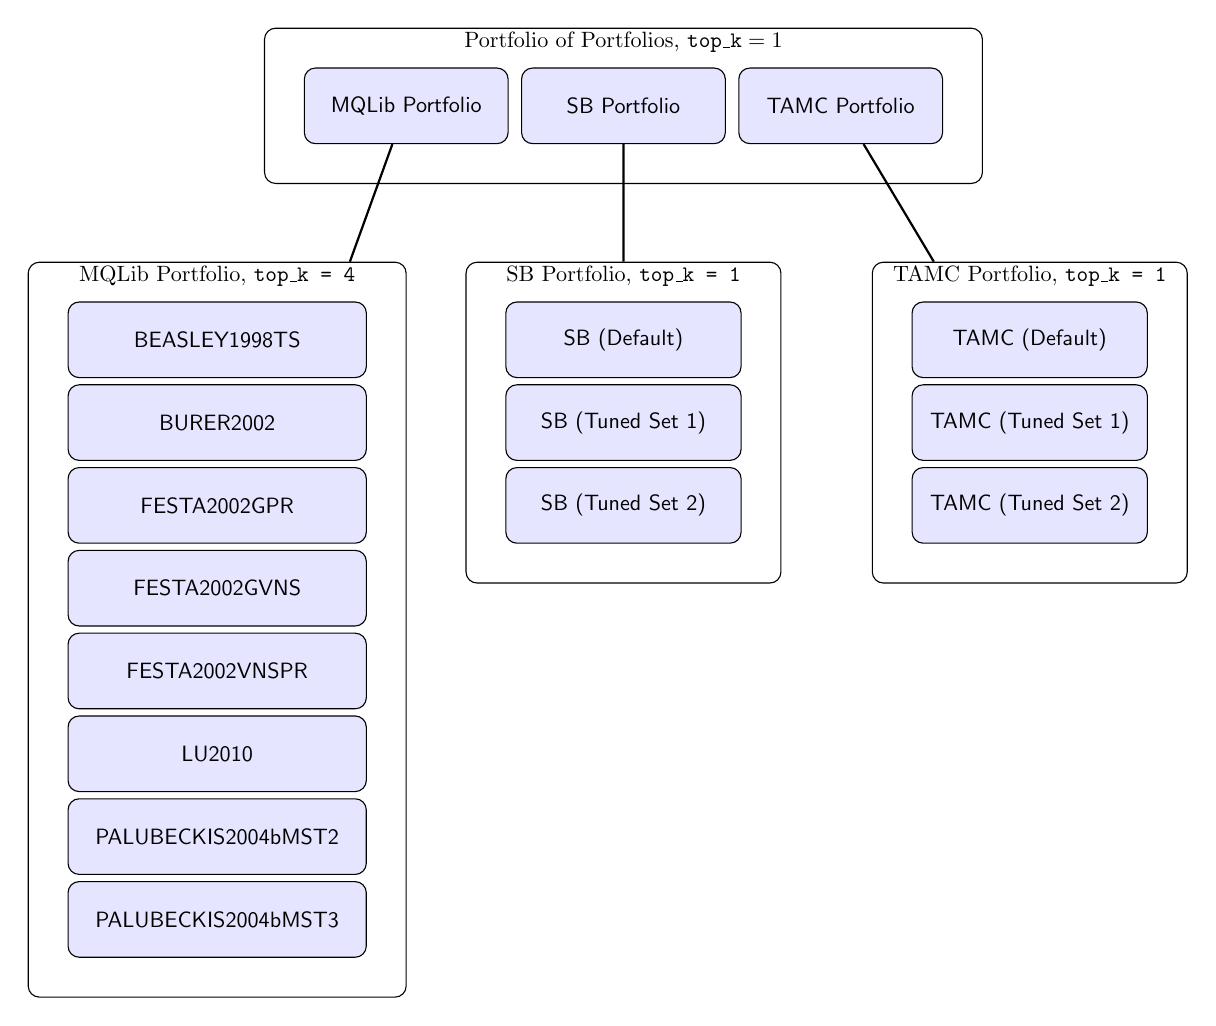
\begin{tikzpicture}[scale=0.8, transform shape,
        data/.style = {
            rectangle,
            draw,
            fill=blue!10,
            rounded corners,
            text width = 4.5cm,
            align = center,
            font = \sffamily,
            minimum height=1.2cm
        },
        portfolio_node/.style 2 args={
            draw,
            solid,
            rounded corners,
            inner sep=0.5cm,
            fit=#1,
            label={[anchor=north, inner sep=2pt]north:{#2}}}
        ]

        \node (ref_mqlib) [data, text width=3cm] {MQLib Portfolio};
        \node (ref_sb) [data, text width=3cm, right=0.2cm of ref_mqlib] {SB Portfolio};
        \node (ref_tamc) [data, text width=3cm, right=0.2cm of ref_sb] {TAMC Portfolio};

        \node[portfolio_node={(ref_mqlib)(ref_sb)(ref_tamc)}{Portfolio of Portfolios, $\texttt{top\_k}=1$}] (pop_class) {};

        \node (mqlib_1) [data, below=2.5cm of ref_mqlib, xshift=-3cm] {BEASLEY1998TS};
        \node (mqlib_2) [data, below=0.1cm of mqlib_1] {BURER2002};
        \node (mqlib_3) [data, below=0.1cm of mqlib_2] {FESTA2002GPR};
        \node (mqlib_4) [data, below=0.1cm of mqlib_3] {FESTA2002GVNS};
        \node (mqlib_5) [data, below=0.1cm of mqlib_4] {FESTA2002VNSPR};
        \node (mqlib_6) [data, below=0.1cm of mqlib_5] {LU2010};
        \node (mqlib_7) [data, below=0.1cm of mqlib_6] {PALUBECKIS2004bMST2};
        \node (mqlib_8) [data, below=0.1cm of mqlib_7] {PALUBECKIS2004bMST3};

        \node (sb_1) [data, text width=3.5cm, below=2.5cm of ref_sb] {SB (Default)};
        \node (sb_2) [data, text width=3.5cm, below=0.1cm of sb_1] {SB (Tuned Set 1)};
        \node (sb_3) [data, text width=3.5cm, below=0.1cm of sb_2] {SB (Tuned Set 2)};

        \node (tamc_1) [data, text width=3.5cm, below=2.5cm of ref_tamc, xshift=3cm] {TAMC (Default)};
        \node (tamc_2) [data, text width=3.5cm, below=0.1cm of tamc_1] {TAMC (Tuned Set 1)};
        \node (tamc_3) [data, text width=3.5cm, below=0.1cm of tamc_2] {TAMC (Tuned Set 2)};

        \node[portfolio_node={(mqlib_1)(mqlib_8)}{MQLib Portfolio, $\texttt{top\_k = 4}$}] (mqlib_class) {};
        \node[portfolio_node={(sb_1)(sb_3)}{SB Portfolio, $\texttt{top\_k = 1}$}] (sb_class) {};
        \node[portfolio_node={(tamc_1)(tamc_3)}{TAMC Portfolio, $\texttt{top\_k = 1}$}] (tamc_class) {};

        \draw[-, thick] (ref_mqlib) -- (mqlib_class);
        \draw[-, thick] (ref_sb) -- (sb_class);
        \draw[-, thick] (ref_tamc) -- (tamc_class);  

    \end{tikzpicture}
\caption{Portfolio of Portfolios configuration. The top level portfolio selects among three sub-portfolios: MQLib Portfolio, SB Portfolio, and TAMC Portfolio. SB and TAMC portfolios include both default and tuned heuristic versions, while the MQLib portfolio consists of the top 8 MQLib heuristics. The \texttt{top\_k} parameter indicates how many heuristics each portfolio can select from its candidates.}
\label{fig:portfolio-of-portfolios}
\end{figure}

All configurations were tested using both Random Forest and XGBoost selectors. Consequently, each flat portfolio was evaluated in two variants: one utilizing Random Forest and the other utilizing XGBoost. Similarly, the hierarchical portfolio (Portfolio of Portfolios) was tested in two configurations, where the top-level selector and all sub-portfolio selectors shared the same model type (either all Random Forest or all XGBoost). This is mark as a suffix in the results tables (e.g., \textit{Portfolio of All Heuristics \textbf{RandomForest}}).


\subsection*{Results on MQLib Test instances}

% script: experiments/experiment4/plot_all_portfolios.jl
\begin{table}[h!]
\centering
\caption{Performance comparison of heuristics and portfolios (bold) on the MQLib test set consisting of 100 instances. The Metaheuristics.jl heuristics are included for reference but were not part of any portfolio and are not counted in the \textit{Worst} column since they would skew the results.\\}
\label{tab:heuristic-performance-experiment3}
\resizebox{\textwidth}{!}{%
\begin{tabular}{l|rrr|rrr}
\toprule
\textbf{Heuristic} & \textbf{Best} & \textbf{Only} & \textbf{Worst} & \textbf{Avg Time (s)} & \textbf{Core Hours} & \textbf{GPU Hours} \\
\midrule
\textbf{Portfolio of Portfolios CPU XGBoost} & 84 & 0 & 27 & 46.535 & 2.0928 & 0.0000 \\
\textbf{Portfolio of All Heuristics RandomForest} & 84 & 0 & 28 & 35.760 & 1.5919 & 0.2574 \\
\textbf{Portfolio of All Heuristics XGBoost} & 82 & 0 & 27 & 40.841 & 1.7453 & 0.4073 \\
\textbf{Portfolio of Portfolios CPU RandomForest} & 82 & 0 & 27 & 43.690 & 2.0537 & 0.0000 \\
\textbf{Portfolio of Portfolios All RandomForest} & 81 & 0 & 27 & 52.088 & 2.0269 & 0.3120 \\
\textbf{MQLib Portfolio RandomForest} & 78 & 0 & 27 & 19.671 & 0.6595 & 0.0000 \\
\textbf{MQLib Portfolio XGBoost} & 76 & 0 & 27 & 19.248 & 0.6479 & 0.0000 \\
\textbf{Portfolio of Portfolios All XGBoost} & 76 & 0 & 27 & 39.356 & 1.2076 & 0.0000 \\
\textbf{SB Portfolio RandomForest} & 59 & 0 & 27 & 45.289 & 1.2580 & 0.7993 \\
\textbf{SB Portfolio XGBoost} & 59 & 0 & 27 & 45.652 & 1.2681 & 0.8056 \\
SB - tuned set 2 & 59 & 0 & 30 & 28.879 & 0.8022 & 0.8022 \\
FESTA2002GPR & 58 & 0 & 31 & 1.377 & 0.0382 & 0.0000 \\
\textbf{TAMC Portfolio RandomForest} & 57 & 0 & 29 & 52.804 & 4.4506 & 0.0000 \\
\textbf{TAMC Portfolio XGBoost} & 57 & 0 & 29 & 51.517 & 4.3005 & 0.0000 \\
FESTA2002GVNS & 56 & 0 & 28 & 1.397 & 0.0388 & 0.0000 \\
PALUBECKIS2004bMST3 & 55 & 0 & 27 & 1.671 & 0.0464 & 0.0000 \\
TAMC default & 53 & 0 & 44 & 27.425 & 3.0473 & 0.0000 \\
SB - tuned set 1 & 48 & 0 & 27 & 36.355 & 1.0099 & 1.0099 \\
BURER2002 & 48 & 0 & 28 & 1.395 & 0.0387 & 0.0000 \\
FESTA2002VNSPR & 46 & 0 & 27 & 1.390 & 0.0386 & 0.0000 \\
LU2010 & 45 & 0 & 30 & 1.483 & 0.0412 & 0.0000 \\
TAMC - tuned set 2 & 44 & 0 & 29 & 39.340 & 4.3711 & 0.0000 \\
SB default & 43 & 0 & 39 & 30.720 & 0.8533 & 0.8533 \\
BEASLEY1998TS & 43 & 0 & 52 & 1.381 & 0.0384 & 0.0000 \\
PALUBECKIS2004bMST2 & 41 & 0 & 33 & 1.387 & 0.0385 & 0.0000 \\
TAMC - tuned set 1 & 39 & 0 & 31 & 16.758 & 1.8620 & 0.0000 \\
\midrule
Metaheuristics.jl - BRKGA & 1 & 0 & -- & 1.918 & 0.0533 & 0.0000 \\
Metaheuristics.jl - PSO & 0 & 0 & -- & 0.195 & 0.0054 & 0.0000 \\
\bottomrule
\end{tabular}
}
\end{table}

Table~\ref{tab:heuristic-performance-experiment3} presents the results on the 100 MQLib test instances. Almost all the Portfolio configurations achieved better results than single heuristics achieved. The only portfolios that underperformed are \textit{TAMC Portfolio RandomForest} and \textit{TAMC Portfolio XGBoost}, which are portfolios costructed from 3 TAMC heuristics, which consist of TAMC heuristics only that performed poorly on the test set.

Interestingly, the best performance was achieved by CPU-only \textit{Portfolio of Portfolios CPU XGBoost}, which achieved 84 best results and 27 worst, almost on par as the second place: \textit{Portfolio of All Heuristics RandomForest}, which contained additionally 3 SB GPU-based heuristics, which individually were among the best ones:  notably the \textit{SB - tuned set 2} achieved the best single-heuristic results among all.

\begin{figure}[h!]
    \centering
    \begin{minipage}{0.8\textwidth}
        \centering
        \includegraphics[width=\linewidth]{../plots/Portfolio_of_Portfolios_CPU_XGBoost_heuristic_usage_histogram.png}
    \end{minipage}
    \par\vspace{0.5cm}
    \begin{minipage}{0.8\textwidth}
        \centering
        \includegraphics[width=\linewidth]{../plots/Portfolio_of_All_Heuristics_RandomForest_heuristic_usage_histogram.png}
    \end{minipage}
    \caption{Heuristic selection histogram for the top 2 best performing portfolios: \textit{Portfolio of Portfolios CPU XGBoost} (top) and \textit{Portfolio of All Heuristics RandomForest} (bottom). The green bars indicate how often a heuristic achieved the best (global) solution across all solvers for a particular instance.}
        \label{fig:heuristic-usage-histograms}
\end{figure}


The top 2 heuristics portfolios were further analyzed by plotting the heuristic selection histograms in Figure~\ref{fig:heuristic-usage-histograms}. The histograms show how many times each heuristic was selected by the portfolio selector across all test instances. The green color indicates the heuristics that achieved the best solution among all heuristics for a given instance. 

For the \textit{Portfolio of Portfolios CPU XGBoost} (top), it contains the sub-portfolios: \textit{MQLib Portfolio RandomForest} and \textit{TAMC Portfolio RandomForest}. The \textit{MQLib Portfolio} was chosen 63 times, with 57 of those selections being the top performing ones, and the \textit{TAMC Portfolio} was selected 37 times, achieving the best solution in 27 instances. Within the \textit{MQLib Portfolio}, the most frequently selected heuristics were \textit{BEASLEY1998TS} and \textit{PALUBECKIS2004\allowbreak bMST3}, while within the \textit{TAMC Portfolio}, the default TAMC heuristic was dominant (The TAMC tuned variants were among the least selected totally). This indicates that the portfolio effectively utilizes the strengths of both MQLib and TAMC heuristics, achieving a better performance than either could alone. This approach could be particularly beneficial in scenarios where computational resources are limited to CPU-only environments. Also notably, this approach was better and faster than the long-running \textit{TAMC Portfolios}, meaning that the additional cheap MQLib heuristics helped the overall performance, in terms of lower energies and faster runtimes.

For the \textit{Portfolio of All Heuristics RandomForest} (bottom), the most frequently selected heuristics were \textit{SB - tuned set 2}, with 30 selections, which showed that the selector found the best performing heuristic among all available ones, but it performed the best only on 19 instances. Interestingly, the \textit{TAMC default} heuristic was selected 25 times, achieving the best solution in 23 instances, indicating that despite its average performance, it still had strengths on certain problem instances. Those 2 heuristics were chosen most of the time (55 out of 100), showing also that the hyperparameter tuning described in Section~\ref{sec:experiment-2-hpo} was effective in improving the performance of the SB heuristic, and thus the total portfolio performance.

Comparing the XGBoost and Random Forest selectors, they both demonstrated similar performance, in terms of results and runtimes: the \textit{Portfolio of All Heuristics RandomForest} was slightly better than the XGBoost variant (84 vs 82 best results), while the \textit{Portfolio of Portfolios CPU XGBoost} outperformed its Random Forest counterpart (84 vs 82 best results). This suggests that both selector types are effective for this problem domain, and the choice between them may depend on specific instance characteristics.

\chapter{Conclusions and Future Work}
The Heuristic Portfolio Framework (HPF), described in Section~\ref{sec:portfolio-concept}, showed that using a group of algorithms guided by machine learning works much better than using single heuristics alone. This was tested on the Quadratic Unconstrained Binary Optimization (QUBO) problem using familiar test data.

A key success was using Bayesian Optimization for Hyperparameter Tuning (see Section~\ref{sec:hyperparameter-tuning-bayesian}). This improved the Simulated Bifurcation (SB) solver, as demonstrated in Section~\ref{sec:experiment-2-hpo}. It also gave the portfolio a wider variety of tools to choose from. For example, the tuned PT-ICM variants performed poorly on their own (see Section~\ref{sec:experiment-2-hpo}). However, when added to the portfolio in Section~\ref{sec:experiment-3-portfolio-configurations}, they became useful.

The best overall result came from a novel design called the \textit{Portfolio of Portfolios} (see Table~\ref{tab:heuristic-performance-experiment3}). This method picked the best mix of MQLib and CPU-based Parallel Tempering (PT-ICM) heuristics. It found the best solution in 84 out of 100 cases on the MQLib test set. This proves that the portfolio successfully combines the different strengths of various solvers.

With the rise of quantum annealers, this portfolio approach could help save resources. It allows expensive quantum machines to be replaced by cheaper, classical heuristics on some runs, when those heuristics are likely to perform better.


\section{Limitations}
The main limitation for the thesis was the compute power. In the MQLib \cite{dunning} thesis the authors paid \textit{\$1,196 (\$32.3 per heuristic)}, while the PT-ICM  \cite{PT_rust} used much more CPU power, not to mention the \texttt{simulated\_bifurcation} package which runs GPU. With more compute, the ML models could be trained on more instances.

The second limitation concerned time measurements and time limits. Since the SB and TAMC heuristics were ran as subprocesses, this limited how I could measure the resource usage. The time measurement was done using wall-clock time, which can be affected by other processes running on the same machine.

The tuning process was also limited by the time budget. Each tuning run had a maximum of 75 iterations, which may not have been enough to fully explore the hyperparameter space, especially for complex heuristics like TAMC.

\section{Future Research}
A component of this thesis that was not explored is the metrics classifier. As I said in Section~\ref{sec:instance-classifier}, the metrics were taken from \cite{dunning} without further exploration. Future research could explore more advanced methods like the ones using transformer architecture to guess the best features \cite{transformer_feature_learning_2025}. The other approach could be to use unsupervised learning to cluster the training instances and then use representative instances from each cluster for tuning different specialized portfolios.

The hyperparameter tuning could be further improved by using instance-specific tuning methods \cite{PIAC_belkhir2017}, where the tuning process learns to predict the best hyperparameters based on the instance features. This could lead to even better performance, as the heuristics would be more finely adapted to each problem.

Also the out-of-distribution generalization could be explored more. In this thesis, the portfolios were tested on instances similar to those used for training. Future work could investigate further which configurations and tuning methods work best on completely different instances.

Finally, the interpretability of the machine learning models offers a way for understanding the relationship between instance features and algorithm performance. An example of a decision tree extracted from the trained Random Forest selector is provided in Appendix~\ref{ch:interpretability}. The XGBoost selectors are also interpretable. Additionally, some newer methods for visualization could be considered \cite{sondag2025clusterbasedrandomforestvisualization}.

\section{Acknowledgements}
I would like to thank \href{https://quantumz.io/}{Quantumz.io} for suggesting this research topic and kickstarting my work. I am also grateful to my supervisors, \textit{Dr. Marcin Szczuka} and \textit{Prof. Łukasz Pawela}, for their guidance and support while writing this thesis.


% Bibliography
\addcontentsline{toc}{chapter}{Bibliography}
\bibliographystyle{plainurl}
\bibliography{bibliography}


% Appendix

\appendix
\chapter{Heuristics Card}
\label{ch:heuristics-card}

% Heuristics Configurations
{
\small % Base font for the table
\setlength{\tabcolsep}{5pt} % Slightly tighter padding to maximize width
\renewcommand{\arraystretch}{1.4} % Increased vertical spacing for the list items

% Adjusted column 1 width to 3.8cm to give more room to the X column
\begin{xltabular}{\textwidth}{>{\raggedright\arraybackslash}p{3.8cm} >{\raggedright\arraybackslash}l >{\raggedright\arraybackslash}X c c}

    % --- Table Header ---
    \caption{Detailed Heuristics Card. This table details the hyperparameter configurations for all algorithms used in the experimental framework.} \label{tab:heuristic-model-card} \\  \toprule
    \textbf{Heuristic} & \textbf{Class} & \textbf{Hyperparameters} & \textbf{Threads} & \textbf{GPU} \\
    \midrule
    \endfirsthead

    % --- Continuation Header ---
    \caption[]{Detailed Heuristics Card (continued)} \\
    \toprule
    \textbf{Heuristic} & \textbf{Class} & \textbf{Hyperparameters} & \textbf{Threads} & \textbf{GPU} \\
    \midrule
    \endhead

    % --- Footer ---
    \midrule
    \multicolumn{5}{r}{\textit{Continued on next page...}} \\
    \endfoot

    % --- Last Footer ---
    \bottomrule
    \endlastfoot

    % --- MQLib Heuristics ---
    BEASLEY1998TS & MQLib & {\footnotesize \textit{Default from paper \cite{dunning}}} & 1 & No \\
    BURER2002 & MQLib & {\footnotesize \textit{Default from paper \cite{dunning}}} & 1 & No \\
    FESTA2002GPR & MQLib & {\footnotesize \textit{Default from paper \cite{dunning}}} & 1 & No \\
    FESTA2002GVNS & MQLib & {\footnotesize \textit{Default from paper \cite{dunning}}} & 1 & No \\
    FESTA2002VNSPR & MQLib & {\footnotesize \textit{Default from paper \cite{dunning}}} & 1 & No \\
    LU2010 & MQLib & {\footnotesize \textit{Default from paper \cite{dunning}}} & 1 & No \\
    PALUBECKIS2004bMST2 & MQLib & {\footnotesize \textit{Default from paper \cite{dunning}}} & 1 & No \\
    PALUBECKIS2004bMST3 & MQLib & {\footnotesize \textit{Default from paper \cite{dunning}}} & 1 & No \\

    \midrule

    % --- Simulated Bifurcation ---
    SB (Default) & Sim. Bifurcation & 
    {\footnotesize 
    \param{time\_step}{0.1} \newline
    \param{pressure\_slope}{0.01} \newline
    \param{heat\_coeff}{0.06} \newline
    \param{agents}{128} \newline
    \param{max\_steps}{10000} \newline
    \param{mode}{``discrete''} \newline
    \param{heated}{false}
    }
    & 1 & Yes \\

    SB (Tuned Set 1) & Sim. Bifurcation & 
    {\footnotesize
    \param{heat\_coeff}{0.173} \newline
    \param{pressure\_slope}{0.01} \newline
    \param{agents}{1973} \newline
    \param{max\_steps}{565} \newline
    \param{mode}{``discrete''} \newline
    \param{time\_step}{0.264} \newline
    \param{heated}{false}
    }
    & 1 & Yes \\

    SB (Tuned Set 2) & Sim. Bifurcation & 
    {\footnotesize
    \param{heat\_coeff}{0.135} \newline
    \param{pressure\_slope}{0.003} \newline
    \param{agents}{1006} \newline
    \param{max\_steps}{811} \newline
    \param{mode}{``discrete''} \newline
    \param{time\_step}{0.645} \newline
    \param{heated}{false}
    }
    & 1 & Yes \\

    \midrule

    % --- Parallel Tempering ---
    TAMC (Default) & Parallel Tempering & 
    {\footnotesize
    \param{lo\_beta}{1.0} \newline
    \param{icm}{true} \newline
    \param{threads}{4} \newline
    \param{num\_sweeps}{2000} \newline
    \param{warmup}{0.5} \newline
    \param{replicas}{2} \newline
    \param{dist}{``Geometric''} \newline
    \param{num\_beta}{32} \newline
    \param{range}{[0.2, 5.0]}
    }
    & 4 & No \\

    TAMC (Tuned Set 1) & Parallel Tempering & 
    {\footnotesize
    \param{lo\_beta}{0.843} \newline
    \param{icm}{true} \newline
    \param{threads}{4} \newline
    \param{num\_sweeps}{204} \newline
    \param{warmup}{0.407} \newline
    \param{replicas}{16} \newline
    \param{dist}{``Geometric''} \newline
    \param{num\_beta}{52} \newline
    \param{range}{[0.309, 4.747]}
    }
    & 4 & No \\

    TAMC (Tuned Set 2) & Parallel Tempering & 
    {\footnotesize
    \param{lo\_beta}{0.813} \newline
    \param{icm}{true} \newline
    \param{threads}{4} \newline
    \param{num\_sweeps}{70} \newline
    \param{warmup}{0.536} \newline
    \param{replicas}{32} \newline
    \param{dist}{``Geometric''} \newline
    \param{num\_beta}{30} \newline
    \param{range}{[0.218, 2.081]}
    }
    & 4 & No \\

    \midrule

    BRKGA (Default) & Metaheuristics.jl & 
    {\footnotesize 
    \texttt{num\_elites} = 20 \newline
    \texttt{num\_mutants} = 10 \newline
    \texttt{num\_offsprings} = 70 \newline
    \texttt{bias} = 0.7
    }
    & 1 & No \\

    PSO (Default) & Metaheuristics.jl & 
    {\footnotesize 
    \texttt{N} = 0 \newline
    \texttt{C1} = 2.0 \newline
    \texttt{C2} = 2.0 \newline
    $\omega$ = 0.8 \newline
    }
    & 1 & No \\

\end{xltabular}
}


% Portfolio Configurations Table
{
\small
\setlength{\tabcolsep}{6pt}
\renewcommand{\arraystretch}{1.5}

\begin{xltabular}{\textwidth}{>{\raggedright\arraybackslash}p{4.5cm} >{\raggedright\arraybackslash}l >{\raggedright\arraybackslash}l >{\raggedright\arraybackslash}X}

    % --- Caption and Label ---
    \caption{Portfolio Configurations. This table shows the architecture and composition of the portfolios evaluated in Experiment 3. \textit{RF} denotes Random Forest and \textit{XGB} denotes XGBoost.} 
    \label{tab:portfolio-configurations} \\
    
    % --- Header ---
    \toprule
    \textbf{Portfolio Name} & \textbf{Selectors} & \textbf{Type} & \textbf{Composition \& Logic} \\
    \midrule
    \endfirsthead

    % --- Continuation Header ---
    \caption[]{Portfolio Configurations (continued)} \\
    \toprule
    \textbf{Portfolio Name} & \textbf{Selectors} & \textbf{Type} & \textbf{Composition \& Logic} \\
    \midrule
    \endhead

    % --- Footer ---
    \midrule
    \multicolumn{4}{r}{\textit{Continued on next page...}} \\
    \endfoot

    % --- Last Footer ---
    \bottomrule
    \endlastfoot

    % --- Content ---
    
    % MQLib Portfolio
    \textbf{MQLib Portfolio} & RF / XGB & Flat & 
    \textbf{Candidates:} 8 MQLib heuristics (BEA98TS, BUR02, FES02GPR, FES02GVNS, FES02VNSPR, LU10, PAL04MST2, PAL04MST3). \newline
    \textbf{Logic:} Selects top 1 heuristic. \\

    % SB Portfolio
    \textbf{SB Portfolio} & RF / XGB & Flat & 
    \textbf{Candidates:} 3 SB variants (Default, Tuned Set 1, Tuned Set 2). \newline
    \textbf{Logic:} Selects top 1 heuristic. Requires GPU. \\

    % TAMC Portfolio
    \textbf{TAMC Portfolio} & RF / XGB & Flat & 
    \textbf{Candidates:} 3 TAMC variants (Default, Tuned Set 1, Tuned Set 2). \newline
    \textbf{Logic:} Selects top 1 heuristic. Multi-threaded. \\

    % Portfolio of All Heuristics
    \textbf{Portfolio of All Heuristics} & RF / XGB & Flat & 
    \textbf{Candidates:} All 14 available heuristics (8 MQLib + 3 SB + 3 TAMC). \newline
    \textbf{Logic:} Selects top 1 heuristic directly from the entire pool. \\

    \midrule

    % Portfolio of Portfolios All
    \textbf{Portfolio of Portfolios All} & RF / XGB & Hierarchical & 
    \textbf{Components:} MQLib Portfolio, SB Portfolio, TAMC Portfolio. \newline
    \textbf{Logic:} Top-level selector chooses a category (MQLib, SB, or TAMC), then executes the selected sub-portfolio. \\

    % Portfolio of Portfolios CPU
    \textbf{Portfolio of Portfolios CPU} & RF / XGB & Hierarchical & 
    \textbf{Components:} 
    1. MQLib Portfolio ($\texttt{top\_k}=4$) \newline
    2. TAMC Portfolio ($\texttt{top\_k}=1$) \newline
    \textbf{Logic:} Designed to saturate 4 CPU cores. Selects between running 4 single-threaded MQLib heuristics or 1 multi-threaded TAMC heuristic. Excludes SB (GPU). \\

\end{xltabular}
}

\chapter{Reproducibility}
\label{ch:reproducibility}

\section*{Code and Data Availability}
The complete source code, along with instructions for reproducing the experiments described in this thesis, is available in the \texttt{QUBOPortfolio.jl} repository hosted at:
\begin{center}
    \url{https://github.com/cezarybednarz/QUBOPortfolio.jl}
\end{center}
The package is implemented in the Julia programming language. The repository structure is organized as follows:
\begin{itemize}
    \item \texttt{experiments/}: Contains the scripts for running the experiments, organized into subfolders \texttt{experiment1}, \texttt{experiment2}, and \texttt{experiment3}.
    \item \texttt{data/}: Stores the selected training and testing datasets.
    \item \texttt{cache/ExecutionResults/}: Contains the raw results generated during execution.
    \item \texttt{cache/portfolios/}: Stores the trained portfolio models.
\end{itemize}

\section*{Environment Setup}
To ensure exact reproducibility, the following software versions and dependencies were used.

\subsection*{Julia Environment}
Julia Version: 1.11.6 \\
Dependencies:
\begin{multicols}{2}
\begin{itemize} \small
    \item \texttt{Arpack v0.5.4}
    \item \texttt{CategoricalArrays v0.10.8}
    \item \texttt{ConcurrentCollections v0.1.1}
    \item \texttt{DBInterface v2.6.1}
    \item \texttt{DataFrames v1.7.0}
    \item \texttt{DecisionTree v0.12.4}
    \item \texttt{Distributions v0.25.119}
    \item \texttt{GLPK v1.2.1}
    \item \texttt{Graphs v1.12.0}
    \item \texttt{Hyperopt v0.5.6}
    \item \texttt{JLD2 v0.5.11}
    \item \texttt{JSON v0.21.4}
    \item \texttt{JuMP v1.23.6}
    \item \texttt{MLJ v0.20.7}
    \item \texttt{MLJBase v1.7.0}
    \item \texttt{MLJDecisionTreeInterface v0.4.2}
    \item \texttt{MLJModels v0.17.9}
    \item \texttt{MLJXGBoostInterface v0.3.13}
    \item \texttt{MQLib v0.4.0}
    \item \texttt{MathOptInterface v1.45.0}
    \item \texttt{Metaheuristics v3.4.0}
    \item \texttt{PProf v3.2.0}
    \item \texttt{Pickle v0.3.5}
    \item \texttt{Plots v1.40.9}
    \item \texttt{PrettyTables v2.4.0}
    \item \texttt{ProgressBars v1.5.1}
    \item \texttt{QUBO v0.3.2}
    \item \texttt{QUBOLib v0.1.0}
    \item \texttt{SQLite v1.6.1}
    \item \texttt{SimpleWeightedGraphs v1.4.0}
    \item \texttt{Statistics v1.11.1}
    \item \texttt{StatsBase v0.34.4}
    \item \texttt{TreeParzen v0.3.4}
    \item \texttt{YAML v0.4.13}
    \item \texttt{ZipFile v0.10.1}
    \item \texttt{LinearAlgebra v1.11.0}
    \item \texttt{Logging v1.11.0}
    \item \texttt{Random v1.11.0}
\end{itemize}
\end{multicols}

\subsection*{External Solvers}
\begin{description}
    \item[Rust Environment] (for TAMC \cite{PT_rust}) \\
    Version: \texttt{1.87.0 (17067e9ac 2025-05-09)}

    \item[Python Environment] (for Simulated Bifurcation \cite{SB_python}) \\
    Version: \texttt{3.10.12} \\
    Dependencies:
    \begin{itemize} \small
        \begin{multicols}{2}
            \item \texttt{filelock==3.13.1}
            \item \texttt{fsspec==2024.6.1}
            \item \texttt{Jinja2==3.1.4}
            \item \texttt{MarkupSafe==3.0.2}
            \item \texttt{mpmath==1.3.0}
            \item \texttt{networkx==3.3}
            \item \texttt{numpy==2.3.3}
            \item \texttt{setuptools==70.2.0}
            \item \texttt{simulated-bifurcation==2.0.0}
            \item \texttt{sympy==1.13.3}
            \item \texttt{tdqm==0.0.1}
            \item \texttt{torch==2.8.0}
            \item \texttt{tqdm==4.67.1}
            \item \texttt{typing\_extensions==4.12.2}
        \end{multicols}  
    \end{itemize}
\end{description}

\chapter{Interpretability: Random Forest Tree Example}
\label{ch:interpretability}

In a Random Forest-based portfolio, a separate Random Forest model is trained for each candidate heuristic (or sub-portfolio) available for selection. Each of these models consists of multiple decision trees. To illustrate the interpretability of these models, I present a single decision tree extracted from the \textit{Portfolio of Portfolios All Heuristics RandomForest} (see Figure~\ref{fig:portfolio-of-portfolios}). This specific Random Forest predicts whether the \textit{TAMC Portfolio RandomForest} will achieve the best result among the three available sub-portfolios: the \textit{SB Portfolio RandomForest}, the \textit{MQLib Portfolio RandomForest}, and the \textit{TAMC Portfolio RandomForest}.

Essentially, this tree provides insight into which structural features are used for determining when the TAMC heuristics are likely to outperform the alternatives.

\begin{figure}[h!]
\centering

\tikzset{
  basic/.style  = {draw, drop shadow, font=\sffamily\footnotesize, rectangle, rounded corners=2pt, align=center, inner sep=3pt},
  root/.style   = {basic, fill=blue!10, text width=4cm}, 
  level-2/.style = {basic, fill=green!10, text width=3.5cm},
  level-3/.style = {basic, fill=yellow!10, text width=2.5cm},
  level-4/.style = {basic, fill=orange!10, text width=2.2cm},
  leaf/.style   = {basic, fill=gray!10, text width=2.0cm, align=center},
  pruned/.style = {basic, fill=orange!10, dashed, text width=2.0cm}
}

\resizebox{\textwidth}{!}{% Resize to fit page width
\begin{forest}
    for tree={
        edge path={
            \noexpand\path[\forestoption{edge}]
                (!u.parent anchor) -- +(0,-10pt) -| (.child anchor)\forestoption{edge label};
        },
        parent anchor=south,
        child anchor=north,
        l sep=10mm, % Vertical separation
        s sep=2mm,  % Sibling separation
        font=\sffamily\footnotesize
    }
    % ROOT NODE
    [Feature 2: "log\_m"\\$< 8.053$ ?, root
        % RIGHT BRANCH (Large/Dense) - Moved to Left
        [Feature 9: "log\_norm\_ev2"\\$< 3.422$ ?, level-2, edge label={node[midway, left, font=\scriptsize]{False}}
            [Feature 37: "avg\_neighbour\_mean"\\$< 0.9166$ ?, level-3
                 [Feature 21: "deg\_mean"\\$< 0.09098$ ?, level-4
                        [True : 5/5, leaf]
                        [Feature 38, pruned]
                 ]
                 [Feature 1: "log\_n"\\$< 8.234$ ?, level-4
                        [True : 16/16, leaf]
                        [False : 1/1, leaf]
                 ]
            ]
            [Feature 16: "weight\_log\_abs\_skew"\\$< 0.004191$ ?, level-3
                 [Feature 25: "deg\_skew\_positive"\\$< 0.5$ ?, level-4
                        [False : 2/2, leaf]
                        [True : 2/2, leaf]
                 ]
                 [Feature 27: "core\_min"\\$< 0.9906$ ?, level-4
                        % The Massive Leaf for Large Graphs
                        [False : 46/46, leaf]
                        [Feature 13, pruned]
                 ]
            ]
        ]
        % LEFT BRANCH (Small/Sparse) - Moved to Right
        [Feature 28: "core\_max"\\$< 0.01938$ ?, level-2, edge label={node[midway, right, font=\scriptsize]{True}}
            [Feature 18: "weight\_log\_kurtosis"\\$< 1.139$ ?, level-3
                 [Feature 7: "mis"\\$< 0.36$ ?, level-4
                        [False : 1/1, leaf]
                        [True : 19/19, leaf]
                 ] 
                 % COLLAPSED NODE: This split into two pruned nodes, so we prune the parent directly.
                 [Feature 13: "weight\_mean"\\$< 126.1$ ?, pruned]
            ]
            [Feature 11: "weight\_min"\\$< -98.5$ ?, level-3
                 [Feature 44: "clust\_max"\\$< 0.2111$ ?, level-4
                        [False : 2/2, leaf]
                        [True : 6/6, leaf]
                 ]
                 % The Massive Leaf for Small Graphs
                 [True : 59/59, leaf]
            ]
        ]
    ]
\end{forest}
}
\caption{Visual representation of a \textit{TAMC Portfolio} decision tree (selected at random) from the \textit{Portfolio of Portfolio All Heuristics} portfolio. The tree splits based on various graph features to determine when the \textit{TAMC Portfolio} is likely to achieve the best result. The tree was pruned to a depth of 4, and some nodes (those reaching levels 5 and beyond) were collapsed for clarity. The ``True''/``False'' on the leaves indicate whether \textit{TAMC Portfolio} was selected as the best heuristic for that path. The numbers after the colons represent the count of instances that followed that path during training (e.g., ``5/5'' means 5 instances reached that leaf, all of which selected \textit{TAMC Portfolio} as the best).}
\label{fig:tree_tamc}
\end{figure}

\end{document}

%%% Local Variables:
%%% mode: latex
%%% TeX-master: t
%%% coding: latin-2
%%% End: